%%%%%%%%%%%%%%%%%%%%%%%%%%%%%%%%%%%%%%%%%%%%%%%%%%%%%%%%%%%%%%%%%%%%%%
% Overleaf (WriteLaTeX) Example: Molecular Chemistry Presentation
%
% Source: http://www.overleaf.com
%
% In these slides we show how Overleaf can be used with standard 
% chemistry packages to easily create professional presentations.
% 
% Feel free to distribute this example, but please keep the referral
% to overleaf.com
% 
%%%%%%%%%%%%%%%%%%%%%%%%%%%%%%%%%%%%%%%%%%%%%%%%%%%%%%%%%%%%%%%%%%%%%%

\documentclass{beamer}

\mode<presentation>
{
  \usetheme{Madrid}       % or try default, Darmstadt, Warsaw, ...
  \usecolortheme{default} % or try albatross, beaver, crane, ...
  \usefonttheme{default}    % or try default, structurebold, ...
  \setbeamertemplate{navigation symbols}{}
  \setbeamertemplate{caption}[numbered]
} 

\usepackage[english]{babel}
\usepackage[utf8x]{inputenc}
\usepackage{chemfig}
\usepackage[version=3]{mhchem}

\usepackage{hyperref}
  \hypersetup{colorlinks=true}
  \hypersetup{urlcolor=blue}
  \hypersetup{linkcolor = .}
\usepackage{xcolor}
\usepackage{siunitx}
  \sisetup{separate-uncertainty = true}
\usepackage{physics}
\usepackage[font=small,labelfont=bf]{caption}
\usepackage{subcaption}
\usepackage[en-GB]{datetime2}
\usepackage{overpic}
\usepackage{feynmp}
\DeclareGraphicsRule{*}{mps}{*}{}

\usepackage{scalerel}
\newcommand{\mylbrace}[2]{\vspace{#2pt}\hspace{6pt}\scaleleftright[\dimexpr5pt+#1\dimexpr0.06pt]{\lbrace}{\rule[\dimexpr2pt-#1\dimexpr0.5pt]{-4pt}{#1pt}}{.}}
\newcommand{\myrbrace}[2]{\vspace{#2pt}\scaleleftright[\dimexpr5pt+#1\dimexpr0.06pt]{.}{\rule[\dimexpr2pt-#1\dimexpr0.5pt]{-4pt}{#1pt}}{\rbrace}\hspace{6pt}}

% Here's where the presentation starts, with the info for the title slide
\title[BESIII Oxford]{BESIII Oxford Group Meeting}
\author{Martin Tat}
\institute{Oxford LHCb}
\date{2nd December 2021}

\titlegraphic{
\includegraphics[width = 4cm, height = 2.8cm]{lhcb.jpg}\hspace{1cm}~%
              
\includegraphics[width = 4cm, height = 2.8cm]{bes3.jpg}}

\begin{document}

\begin{frame}
  \titlepage
\end{frame}

% These three lines create an automatically generated table of contents.
%\begin{frame}{Outline}
%  \tableofcontents
%\end{frame}

\section{Intorduction}
\begin{frame}{Introduction}
  \begin{itemize}
    \setlength\itemsep{1.3em}
    \item{Strong-phase analysis of $D^0\to K^+K^-\pi^+\pi^-$}
    \item{Measure $c_i$, $s_i$ (and $K_i$) using double-tags}
    \item{Strategy:}
    \begin{enumerate}
      \item{Determine single tag yields for normalization}
      \item{Determine $KK\pi\pi$ vs flavour tag yields to obtain $K_i$}
      \item{Determine $KK\pi\pi$ vs CP and self-conjugate tag yields}
      \item{Maximum likelihood fit to obtain $c_i$ and $s_i$}
    \end{enumerate}
    \item{Focused a lot on covering \textit{all} tag modes previously...}
    \item{Current plan is to first obtain $K_i$ and make sure everything works}
    \item{Then run toys with yields extrapolated to $\SI{20}{\per\femto\barn}$ in fit to $c_i$ and $s_i$}
  \end{itemize}
\end{frame}

\section{Previous work}
\begin{frame}{Previous work (before May 2021)}
  \begin{itemize}
    \setlength\itemsep{2em}
    \item{Fitted single tag $\Delta E$ distributions}
    \begin{itemize}
      \item{Double Gaussian + 2nd order polynomial}
      \item{Apply cut at $\pm3\sigma$}
    \end{itemize}
    \item{Fitted single tag $m_{\rm BC}$ distributions}
    \begin{itemize}
      \item{Signal shape from MC, Argus for combinatorial background, Gaussian for peaking backgrounds}
      \item{Fit quality very poor in flavour tag modes because of higher statistics}
    \end{itemize}
    \item{Double tag yield using sideband subtraction (same as $K_SKK$ strong-phase analysis)}
  \end{itemize}
\end{frame}

\section{New \texorpdfstring{$\Delta E$}{DeltaE} fits}
\begin{frame}{New $\Delta E$ fits}
  \begin{itemize}
    \setlength\itemsep{2em}
    \item{Signal: Double Gaussian}
    \item{Background: Chebychev polynomials of arbitrary order for two- and three-body modes}
    \item{For $KK\pi\pi$ and $K\pi\pi\pi$ use two independent polynomials on each side of $\Delta E = 0$}
  \end{itemize}
\end{frame}

\begin{frame}{New $\Delta E$ fits}
  \begin{figure}
    \centering
    \begin{subfigure}{0.38\textwidth}
      \centering
      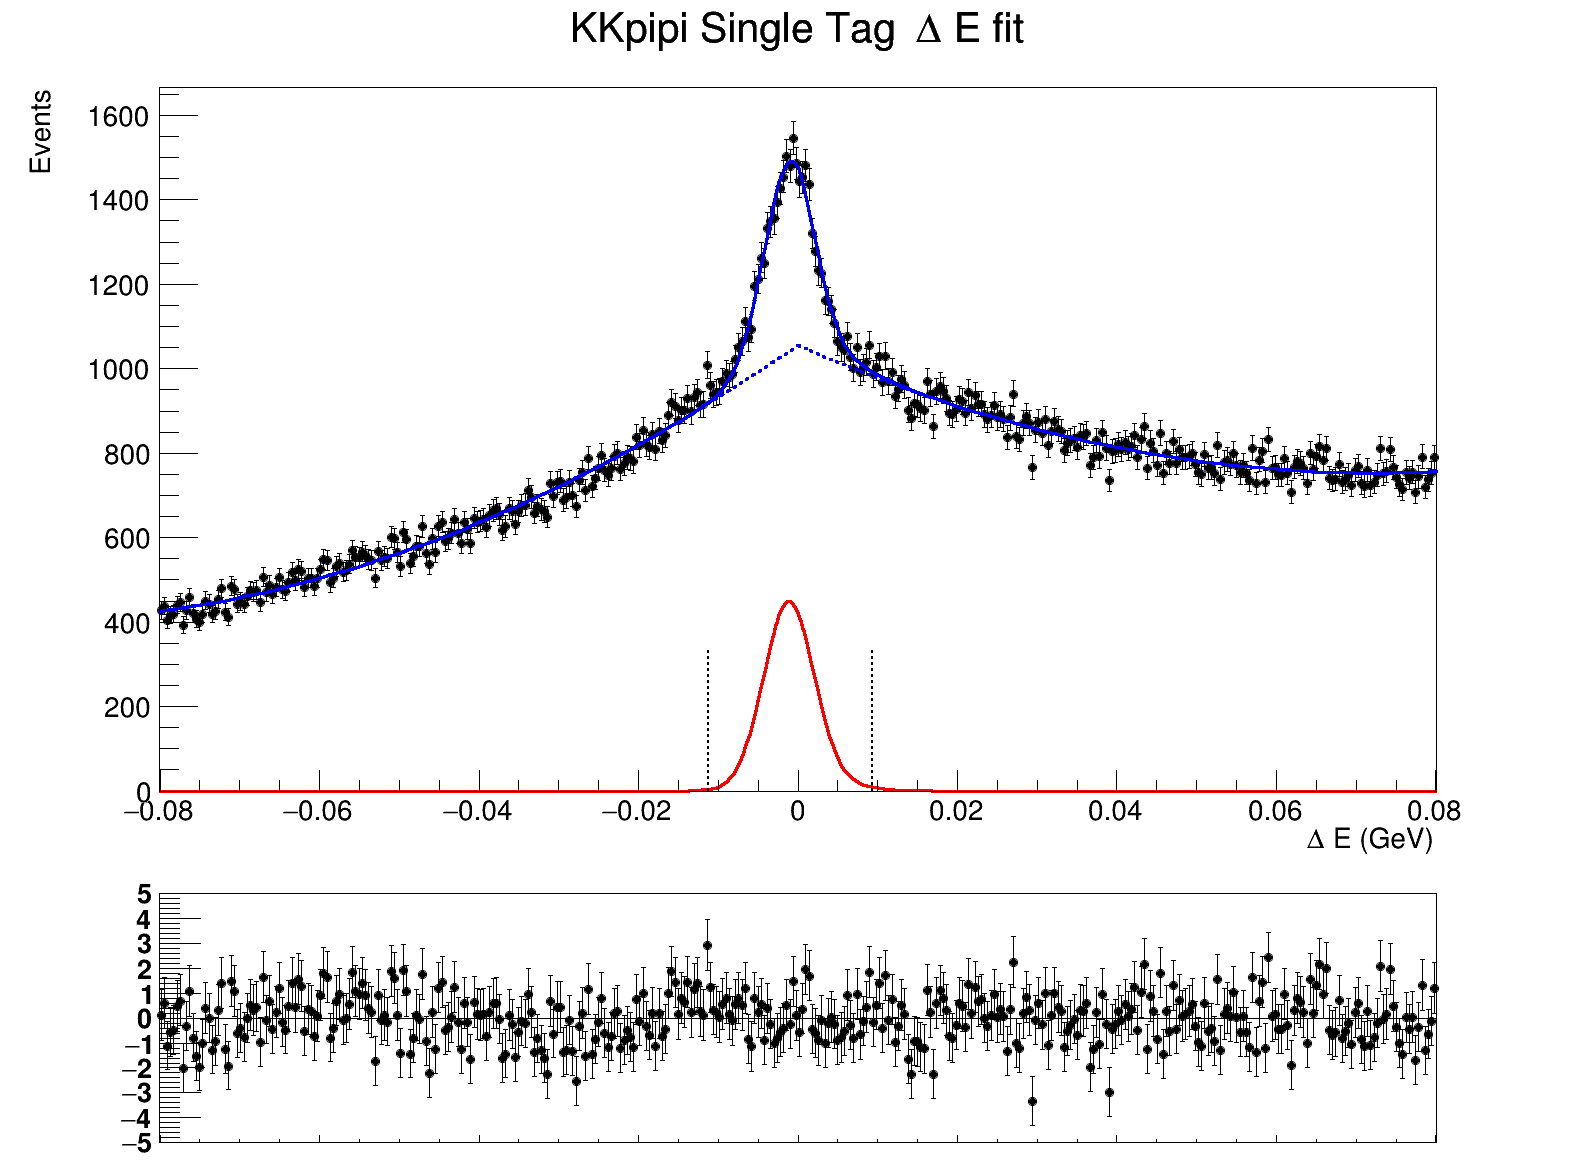
\includegraphics[width=\textwidth]{Plots/KKpipi_SingleTag_DeltaE_Plot.png}
      \caption{$KK\pi\pi$}
    \end{subfigure}%
    \begin{subfigure}{0.38\textwidth}
      \centering
      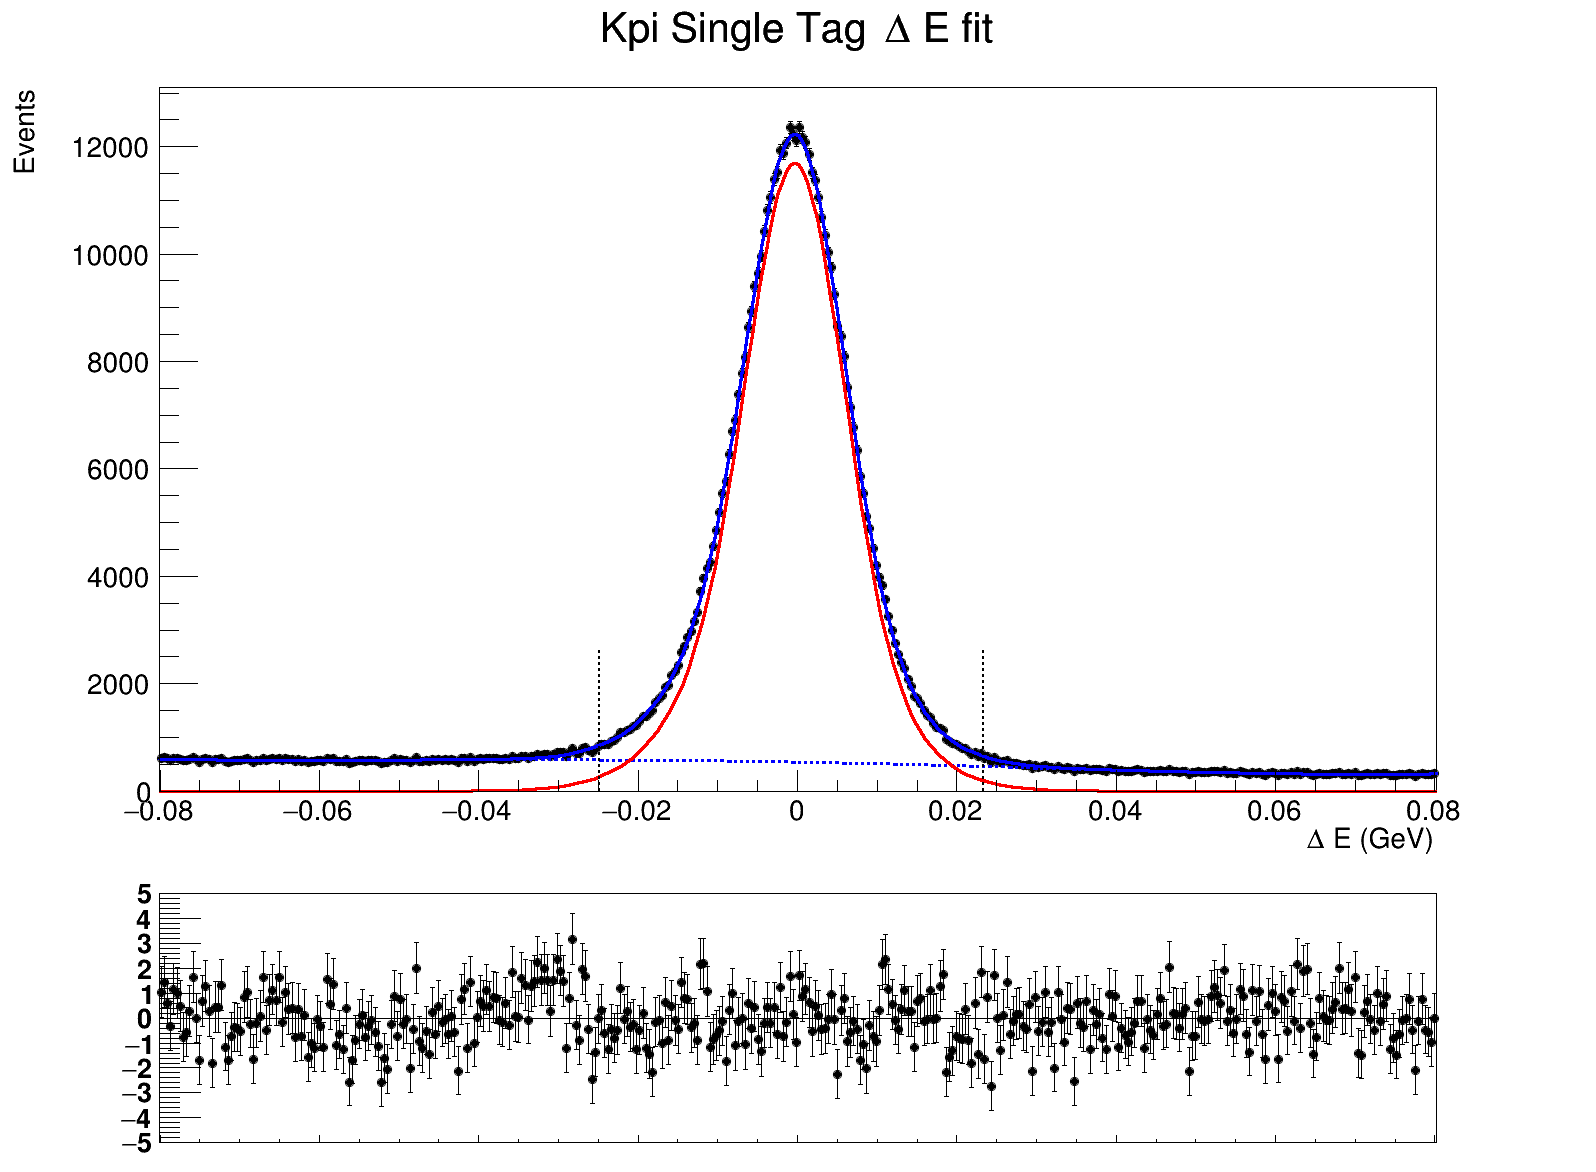
\includegraphics[width=\textwidth]{Plots/Kpi_SingleTag_DeltaE_Plot.png}
      \caption{$K\pi$}
    \end{subfigure}
    \begin{subfigure}{0.38\textwidth}
      \centering
      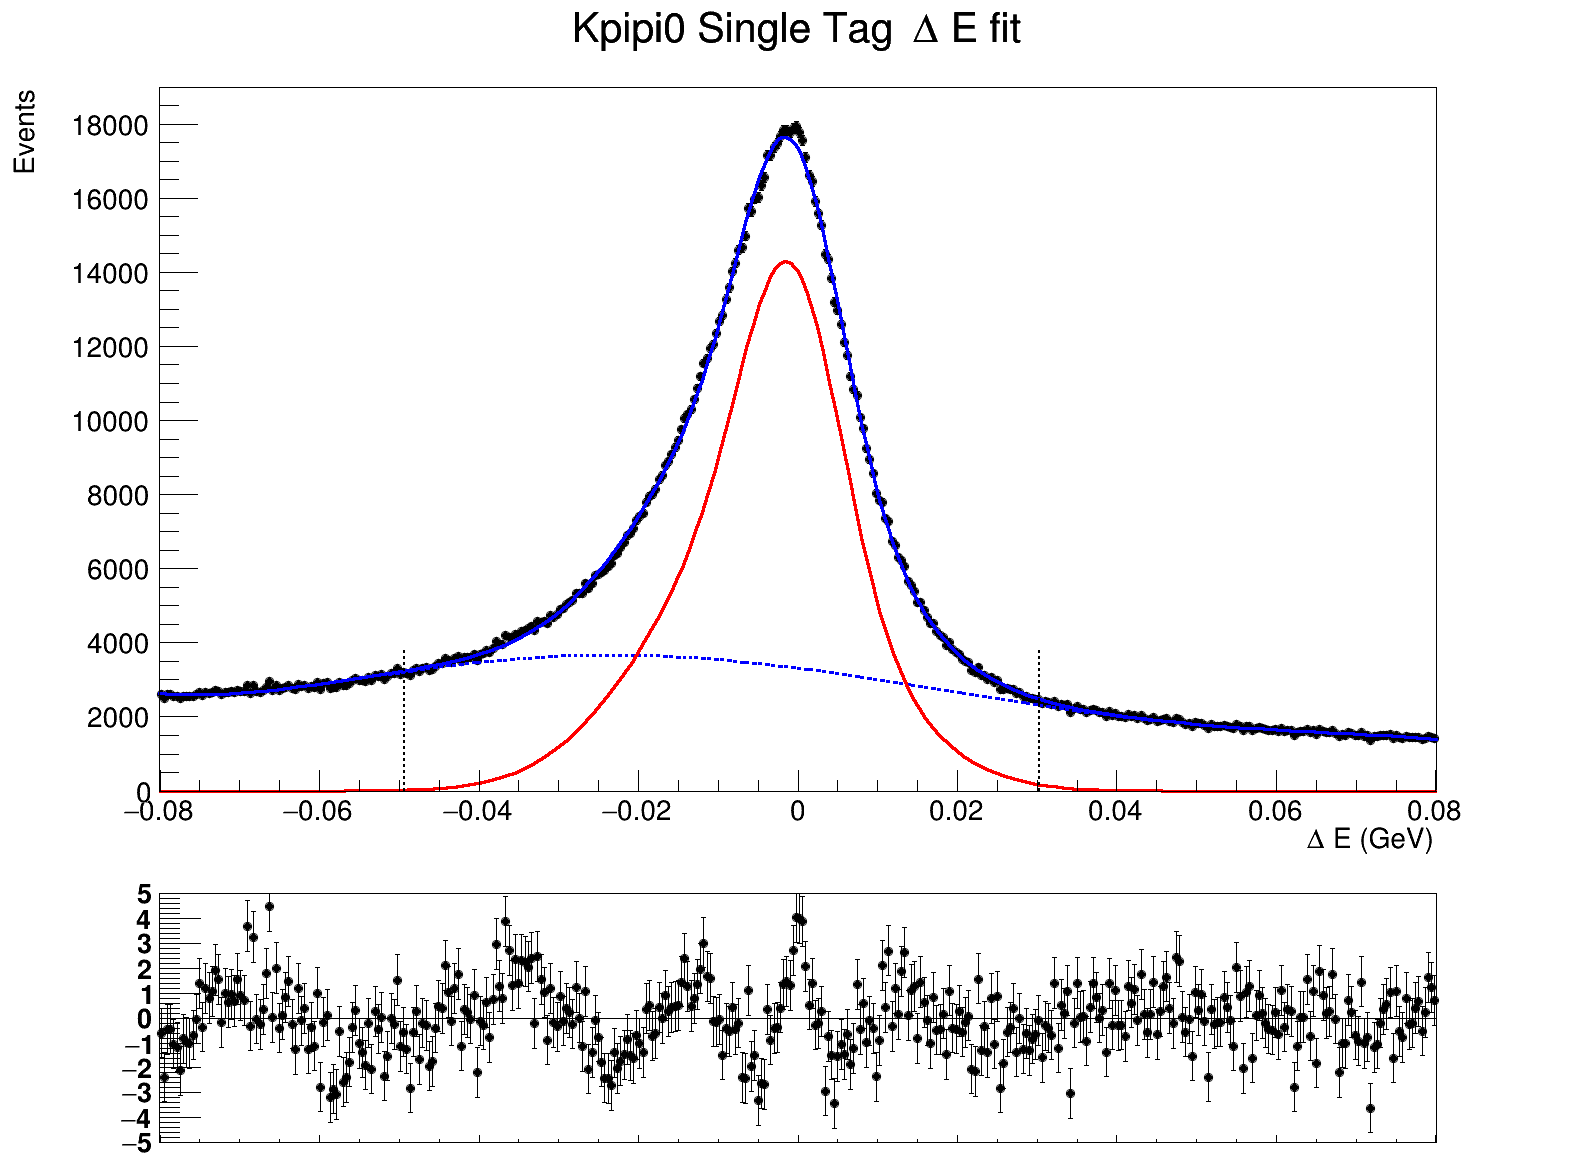
\includegraphics[width=\textwidth]{Plots/Kpipi0_SingleTag_DeltaE_Plot.png}
      \caption{$K\pi\pi^0$}
    \end{subfigure}%
    \begin{subfigure}{0.38\textwidth}
      \centering
      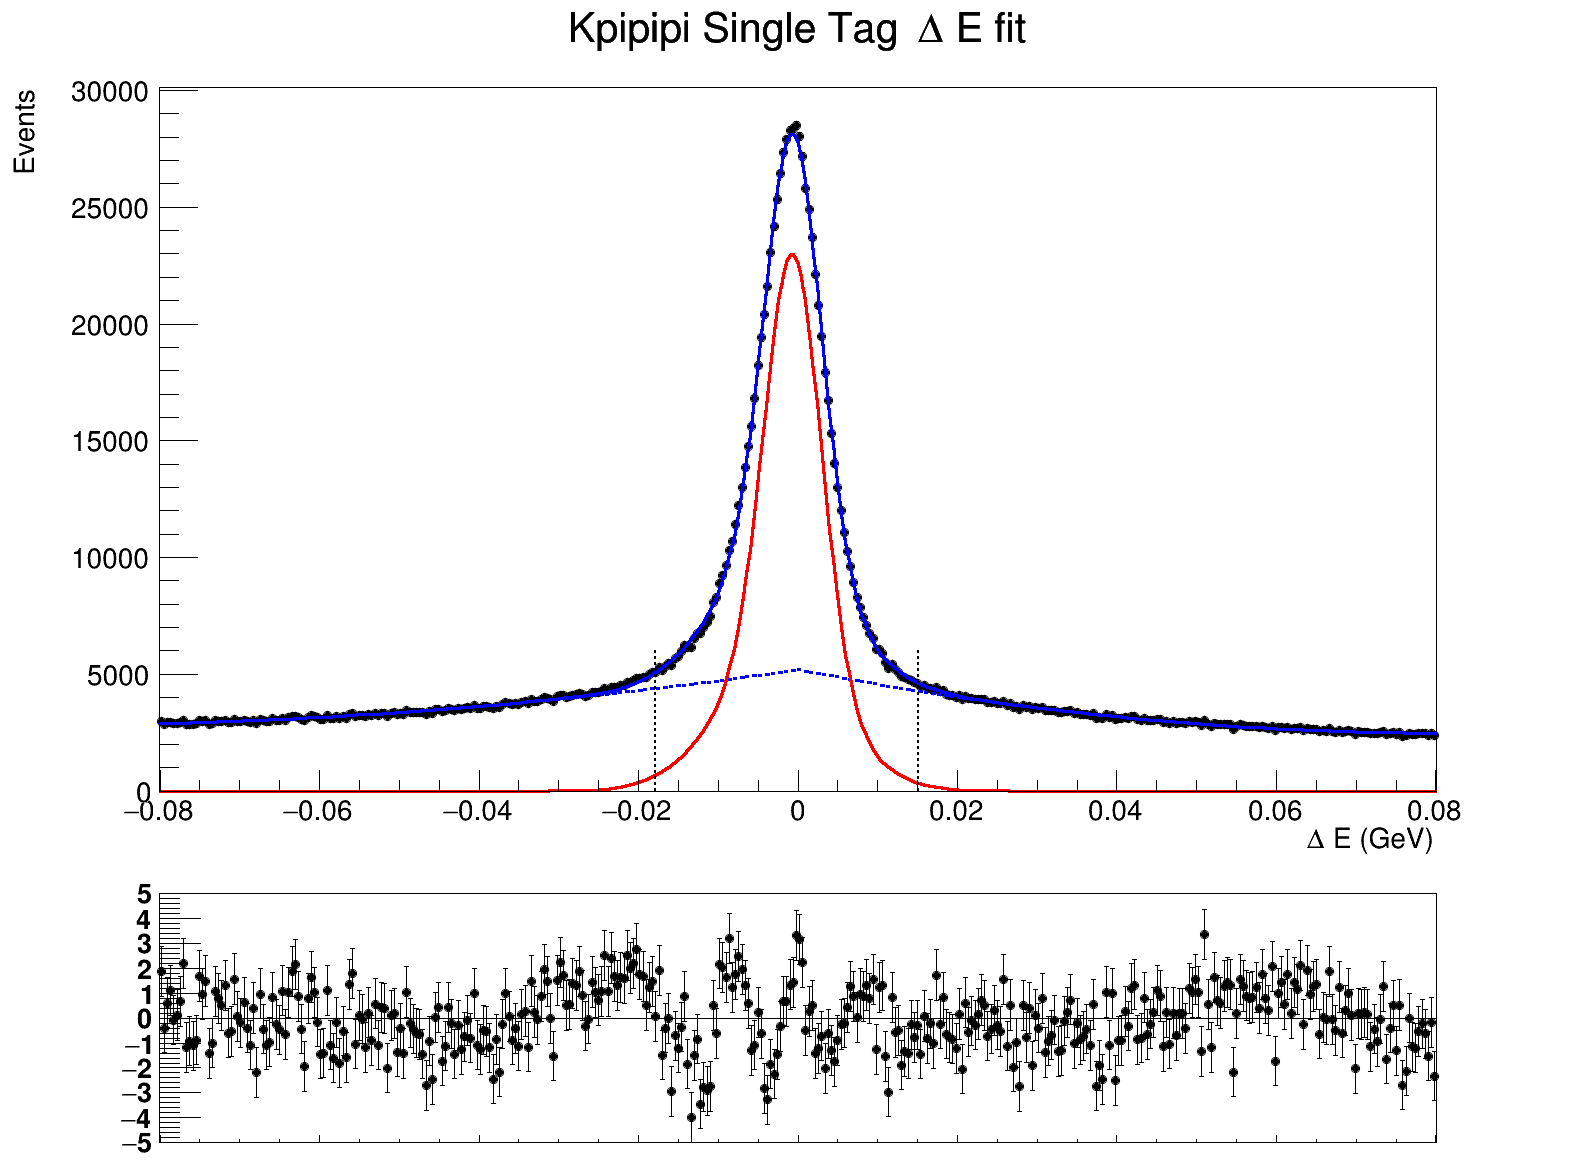
\includegraphics[width=\textwidth]{Plots/Kpipipi_SingleTag_DeltaE_Plot.png}
      \caption{$K\pi\pi\pi$}
    \end{subfigure}
  \end{figure}
\end{frame}

\section{New single tag \texorpdfstring{$m_{\rm BC}$}{MBC} fits}
\begin{frame}{New single tag $m_{\rm BC}$ fits}
  \begin{itemize}
    \setlength\itemsep{2em}
    \item{Signal: Signal MC shape (after truth matching)}
    \item{Resolution: Convolve with double Gaussian}
    \item{Combinatorial background: Argus shape}
    \item{Can add arbitrary shapes for peaking backgrounds}
    \item{New strategy for peaking backgrounds:}
    \begin{enumerate}
      \item{Identify backgrounds with inclusive MC}
      \item{Generate signal MC and fit shape to this sample}
      \item{Calculate yield using relative efficiencies and branching fractions}
    \end{enumerate}
  \end{itemize}
\end{frame}

\begin{frame}{New single tag $m_{\rm BC}$ fits}
  \begin{figure}
    \centering
    \begin{subfigure}{0.49\textwidth}
      \centering
      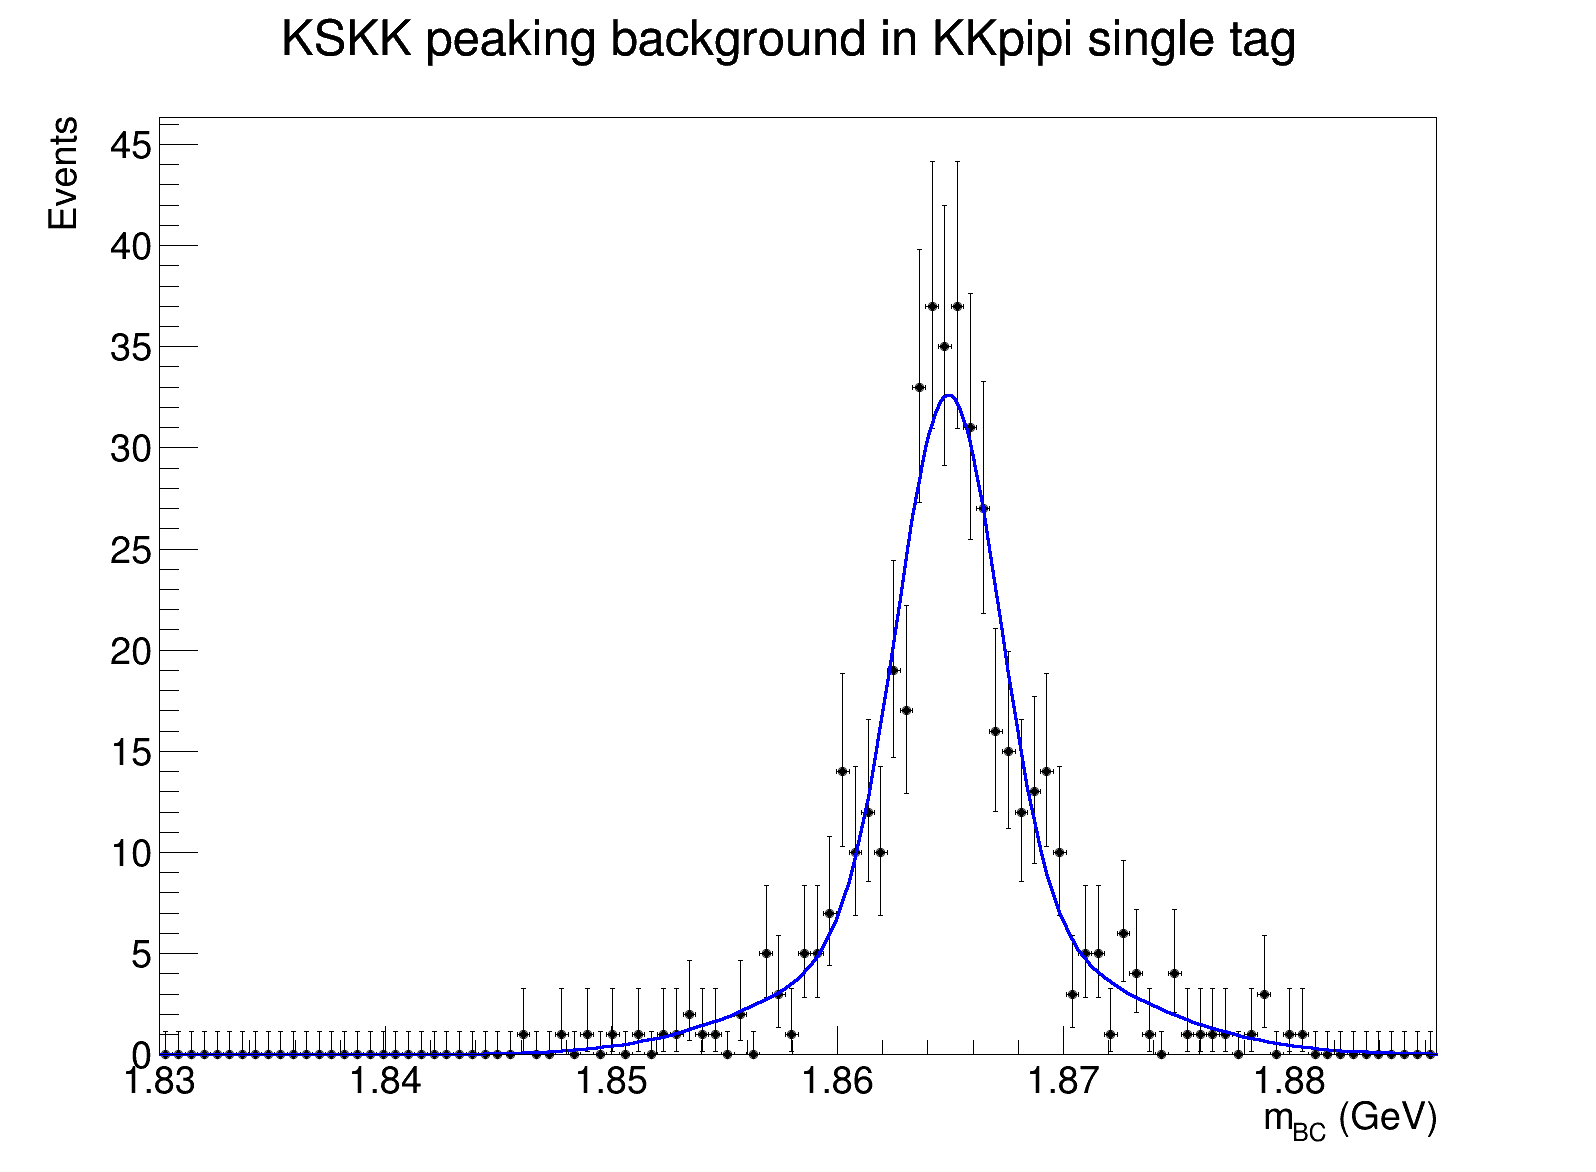
\includegraphics[width=\textwidth]{Plots/KSKKtoKKpipi_Fit.png}
      \caption{$K_SKK\to KK\pi\pi$}
    \end{subfigure}%
    \begin{subfigure}{0.49\textwidth}
      \centering
      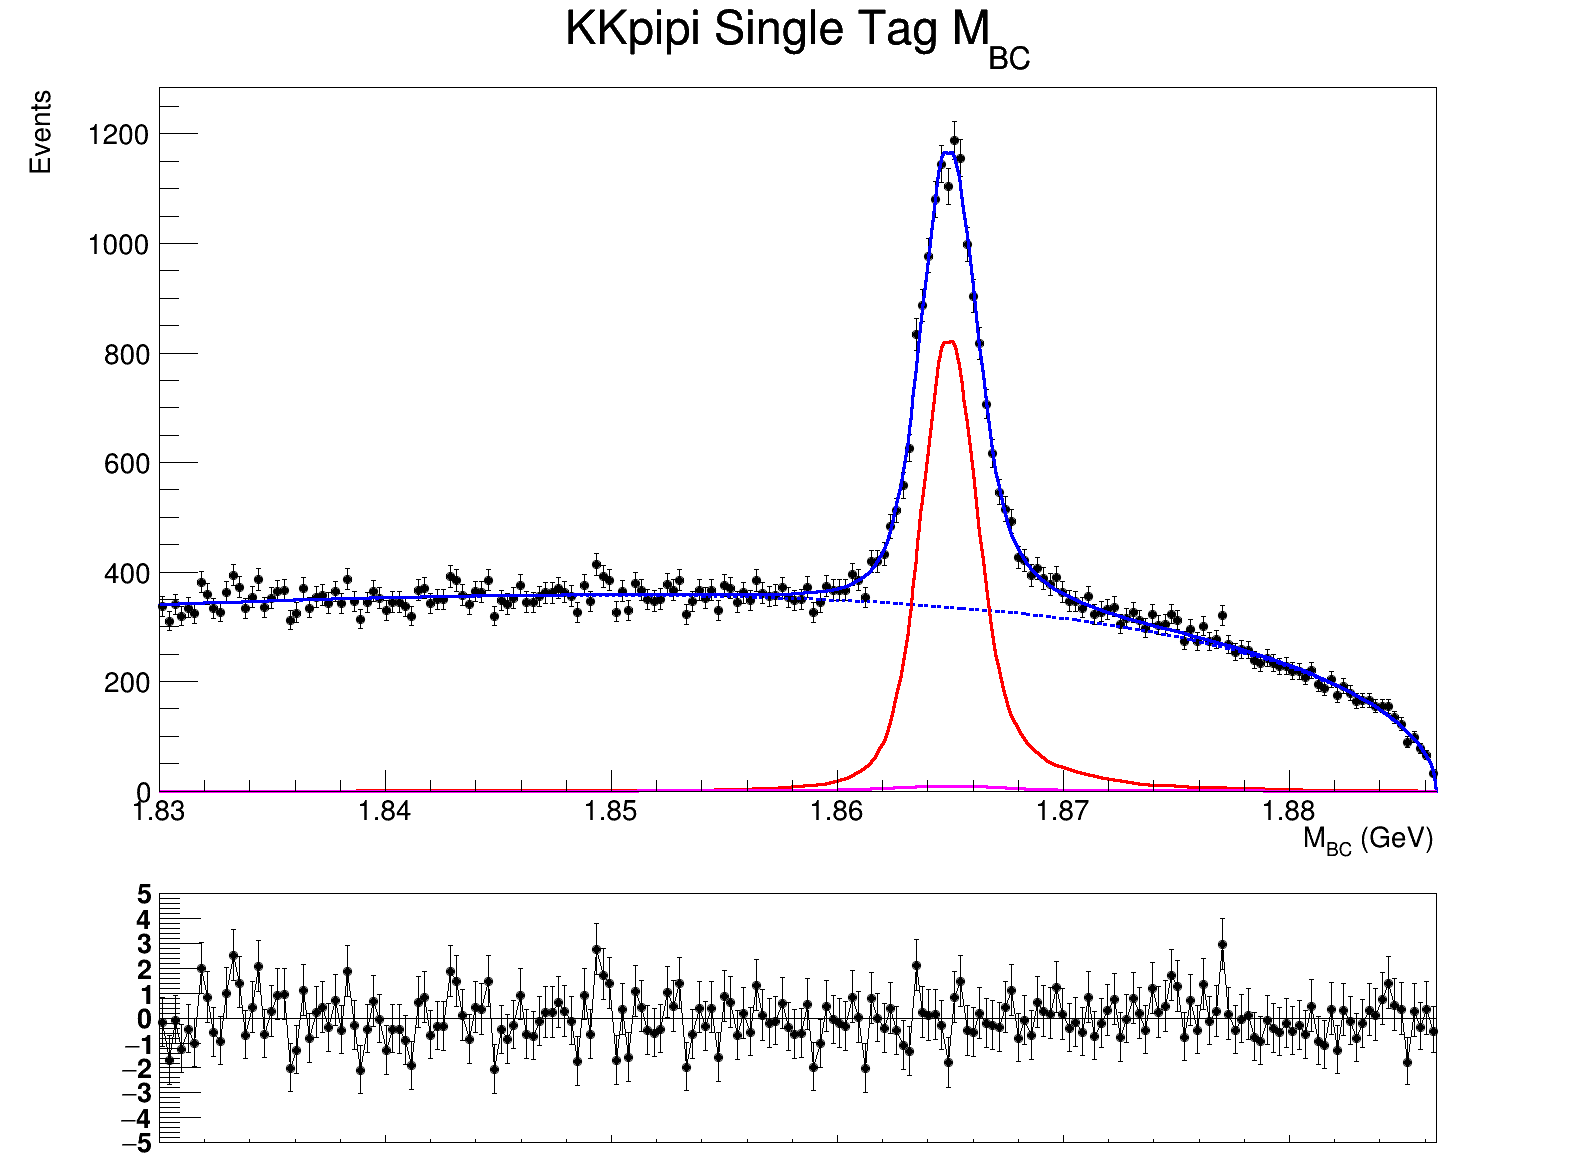
\includegraphics[width=\textwidth]{Plots/KKpipi_SingleTag_MBC_Plot.png}
      \caption{$KK\pi\pi$ $m_{\rm BC}$ fit}
    \end{subfigure}
  \end{figure}
  \begin{center}
    Yield: $\SI{10821(198)}{}$
  \end{center}
\end{frame}

\begin{frame}{New single tag $m_{\rm BC}$ fits}
  \begin{figure}
    \centering
    \begin{subfigure}{0.38\textwidth}
      \centering
      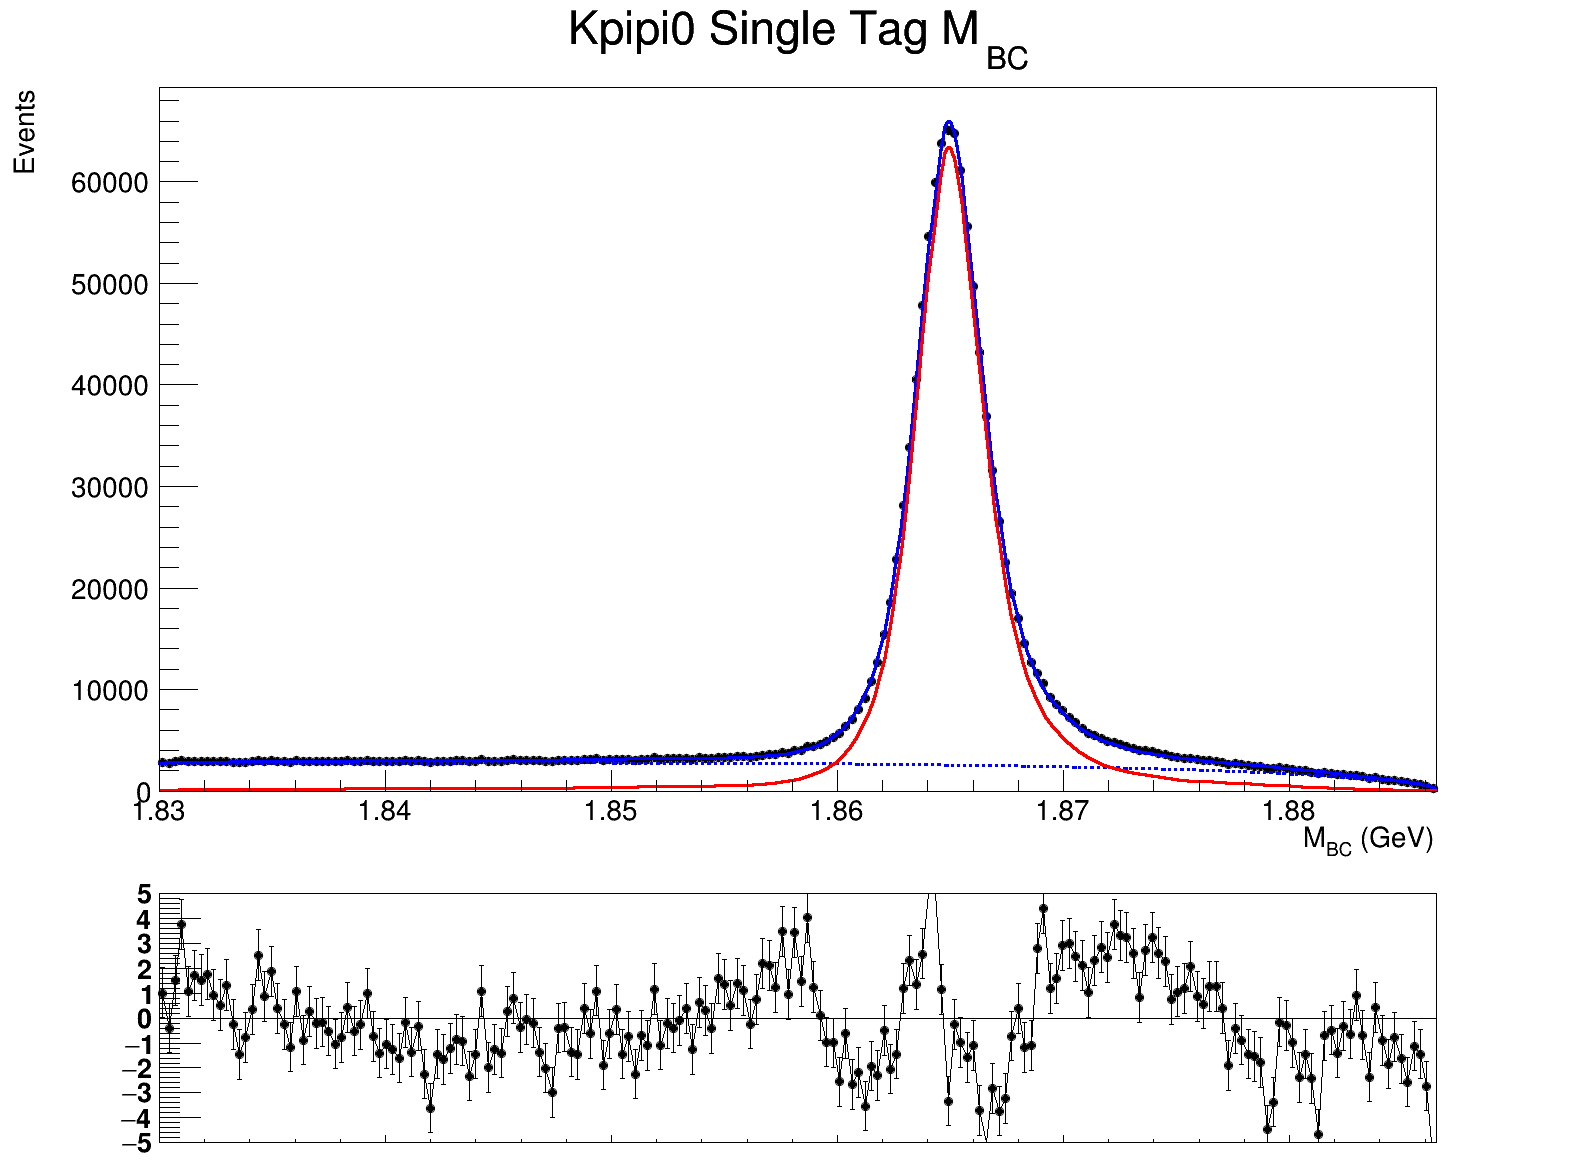
\includegraphics[width=\textwidth]{Plots/Kpipi0_SingleTag_MBC_Plot.png}
      \caption{$K\pi\pi^0$ $m_{\rm BC}$ fit}
    \end{subfigure}
    \begin{subfigure}{0.38\textwidth}
      \centering
      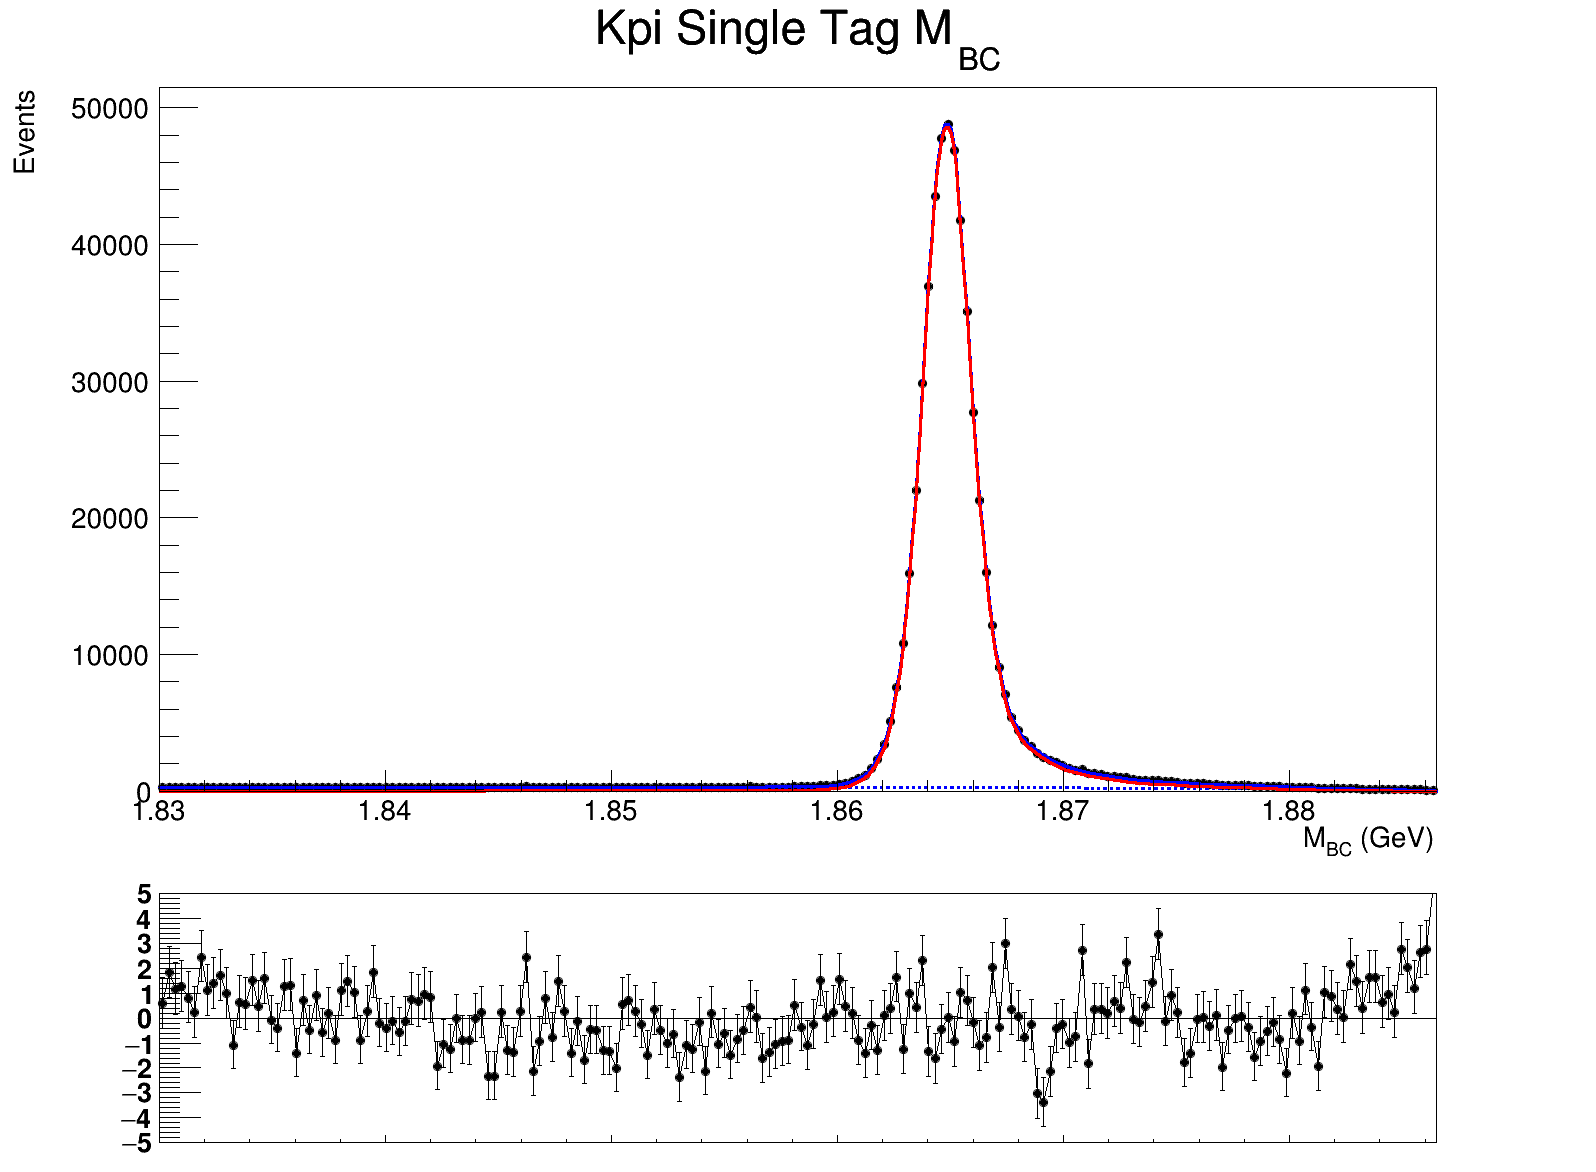
\includegraphics[width=\textwidth]{Plots/Kpi_SingleTag_MBC_Plot.png}
      \caption{$K\pi$ $m_{\rm BC}$ fit}
    \end{subfigure}%
    \begin{subfigure}{0.38\textwidth}
      \centering
      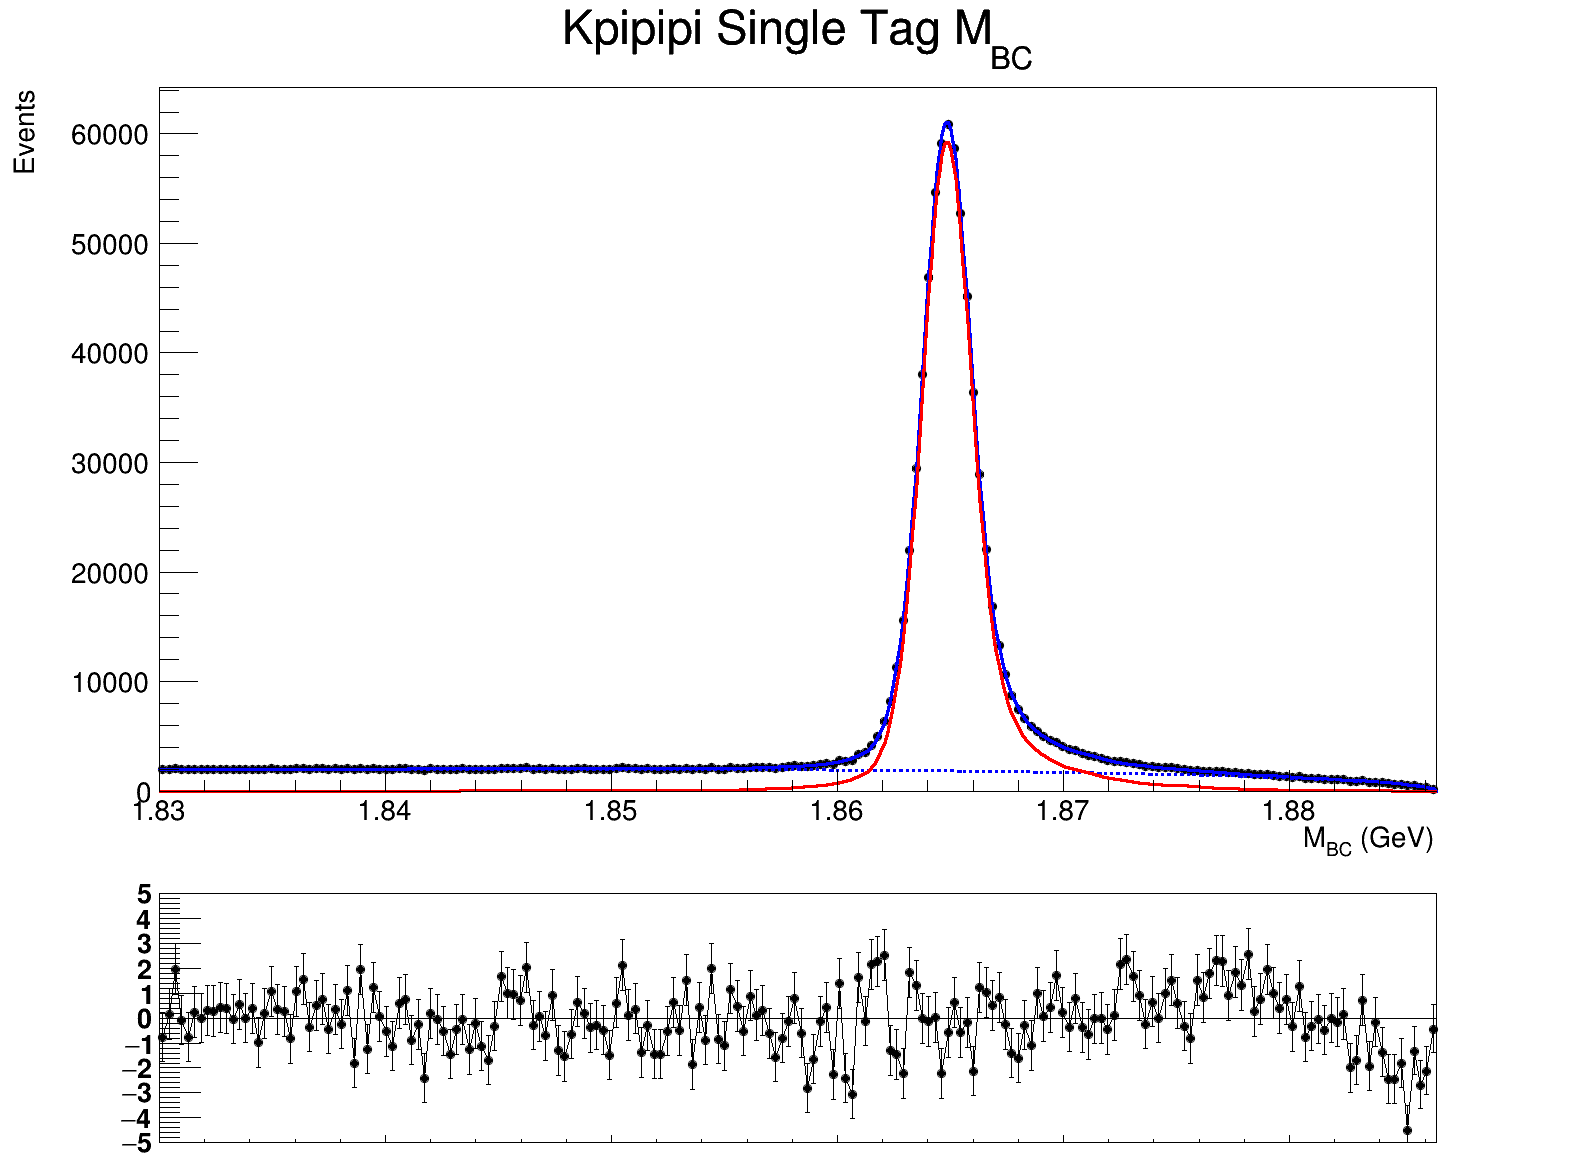
\includegraphics[width=\textwidth]{Plots/Kpipipi_SingleTag_MBC_Plot.png}
      \caption{$K\pi\pi\pi$ $m_{\rm BC}$ fit}
    \end{subfigure}
  \end{figure}
\end{frame}

\section{Double tag yield simultaneous fit}
\begin{frame}{Double tag yield simultaneous fit ($KK\pi\pi$ vs $K\pi$)}
  \begin{itemize}
    \setlength\itemsep{1.5em}
    \item{Should have enough events to perform fit of $KK\pi\pi$ $m_{\rm BC}$}
    \begin{itemize}
      \item{Same strategy as $\pi\pi\pi\pi$ strong-phase analysis}
      \item{Use $2\times 4$ bins for now}
      \item{Scrap sideband subtraction}
    \end{itemize}
    \item{Fit shapes:}
    \begin{itemize}
      \item{Signal shape: Signal MC shape (after truth matching)}
      \item{Resolution: Single Gaussian}
      \item{Combinatorial background: Argus shape}
    \end{itemize}
    \item{Fit strategy:}
    \begin{enumerate}
      \item{For each double tag mode, perform simultaneous fit of all bins}
      \item{Float signal and combinatoria yield in each bin}
      \item{Gaussian shape and Argus slope are floated}
      \item{Then fix all shapes and any combinatorial background less than $0.5$}
      \item{Fit a second time to obtain accurate signal yields in each bin}
    \end{enumerate}
  \end{itemize}
\end{frame}

\begin{frame}{Double tag yield simultaneous fit ($KK\pi\pi$ vs $K\pi$)}
  \begin{figure}
    \centering
    \begin{subfigure}{0.38\textwidth}
      \centering
      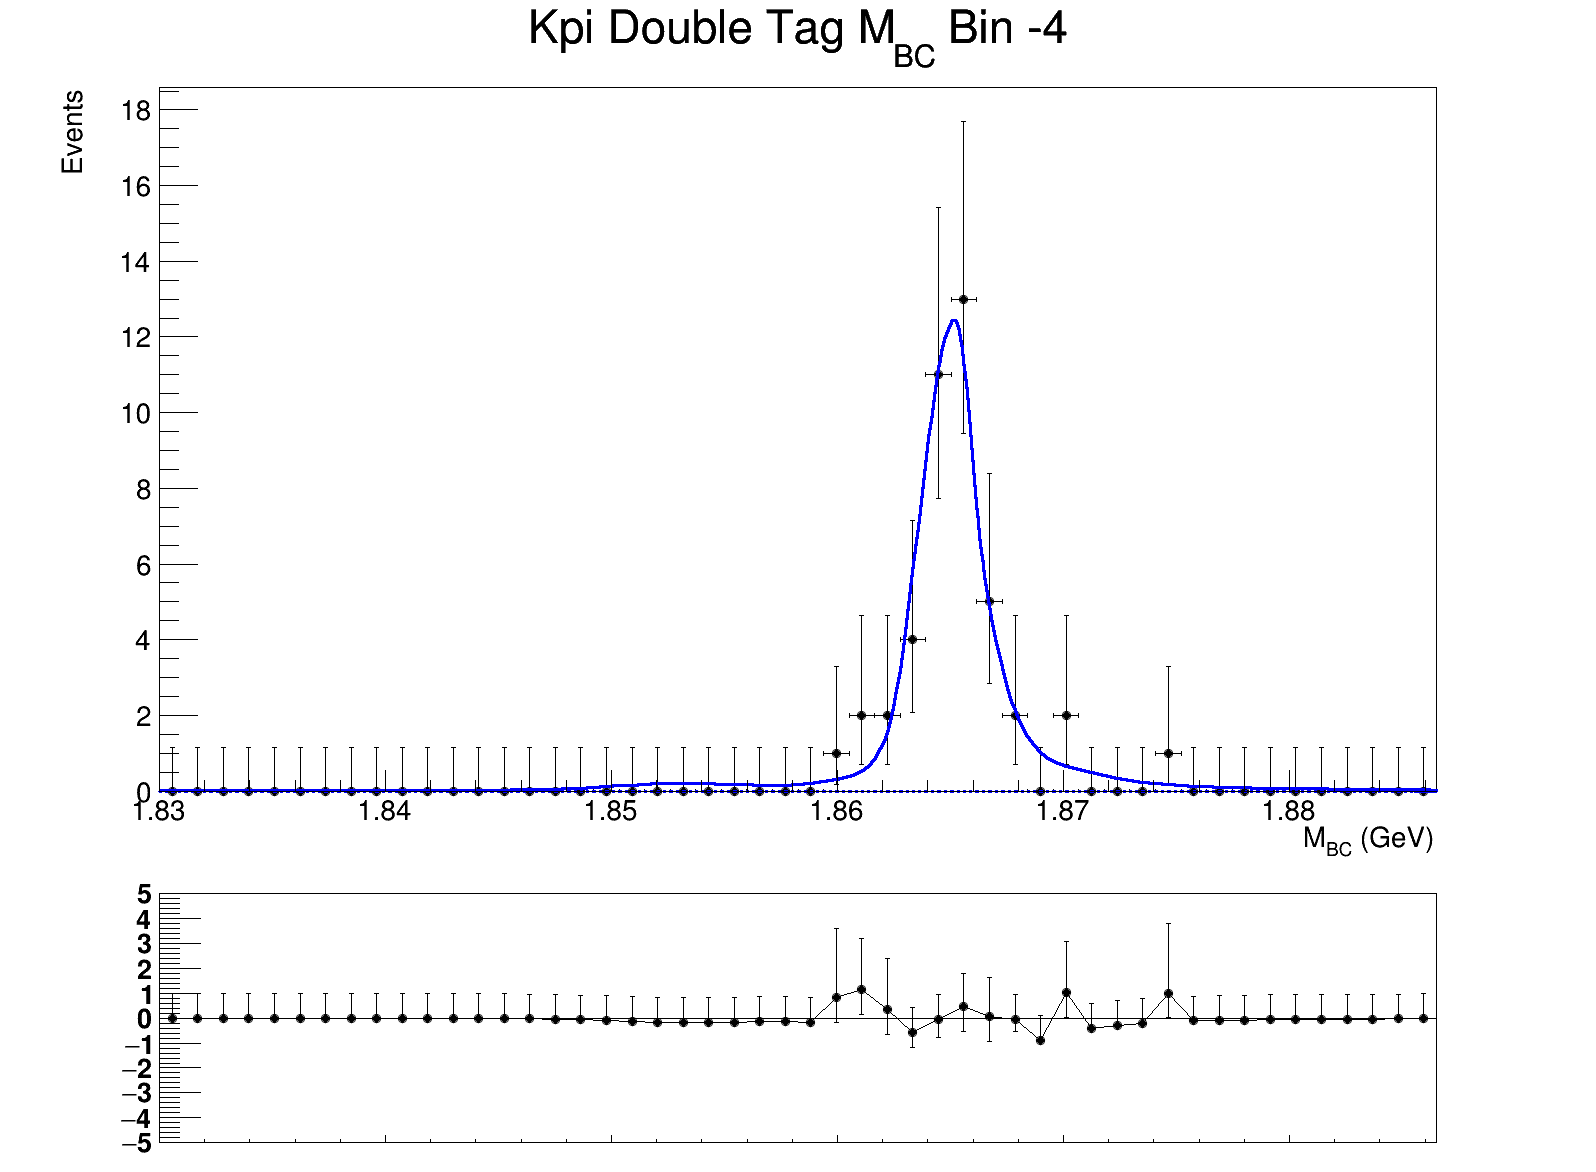
\includegraphics[width=\textwidth]{Plots/DoubleTagYield_DoubleTag_Flavour_KKpipi_vs_Kpi_SignalBinM4_TagBin0.png}
      \caption{Bin $-4$}
    \end{subfigure}%
    \begin{subfigure}{0.38\textwidth}
      \centering
      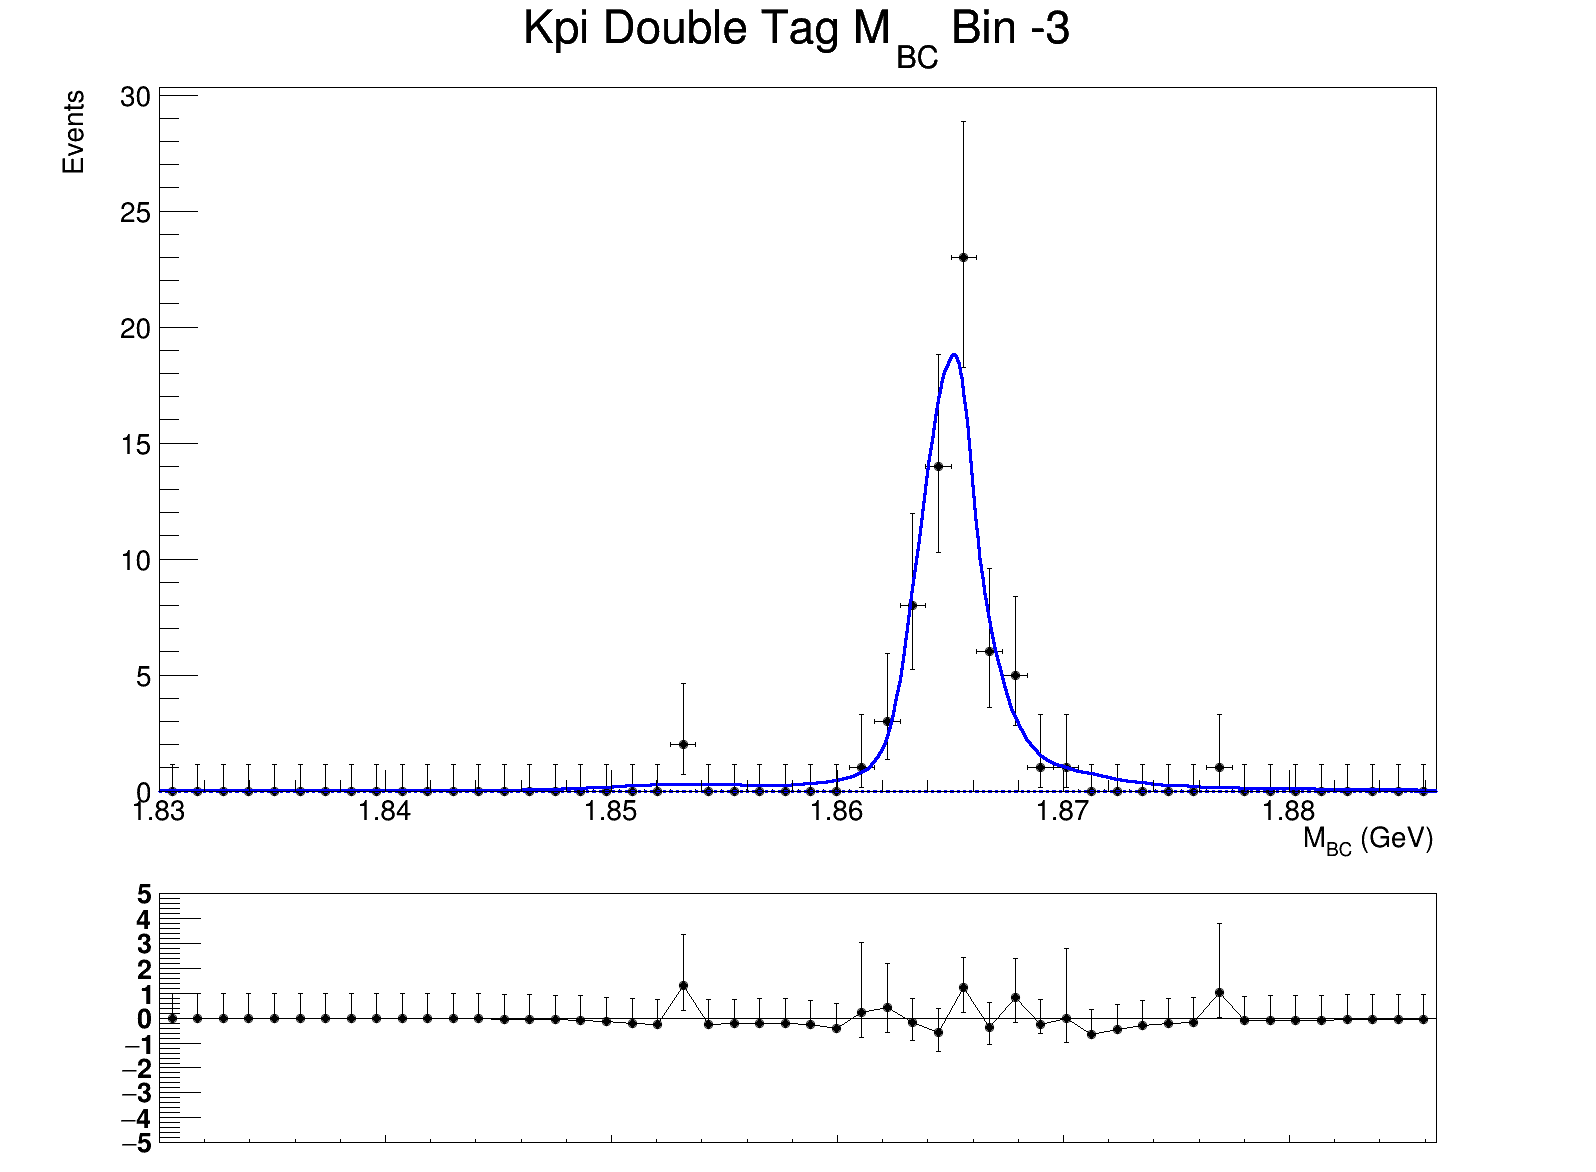
\includegraphics[width=\textwidth]{Plots/DoubleTagYield_DoubleTag_Flavour_KKpipi_vs_Kpi_SignalBinM3_TagBin0.png}
      \caption{Bin $-3$}
    \end{subfigure}
    \begin{subfigure}{0.38\textwidth}
      \centering
      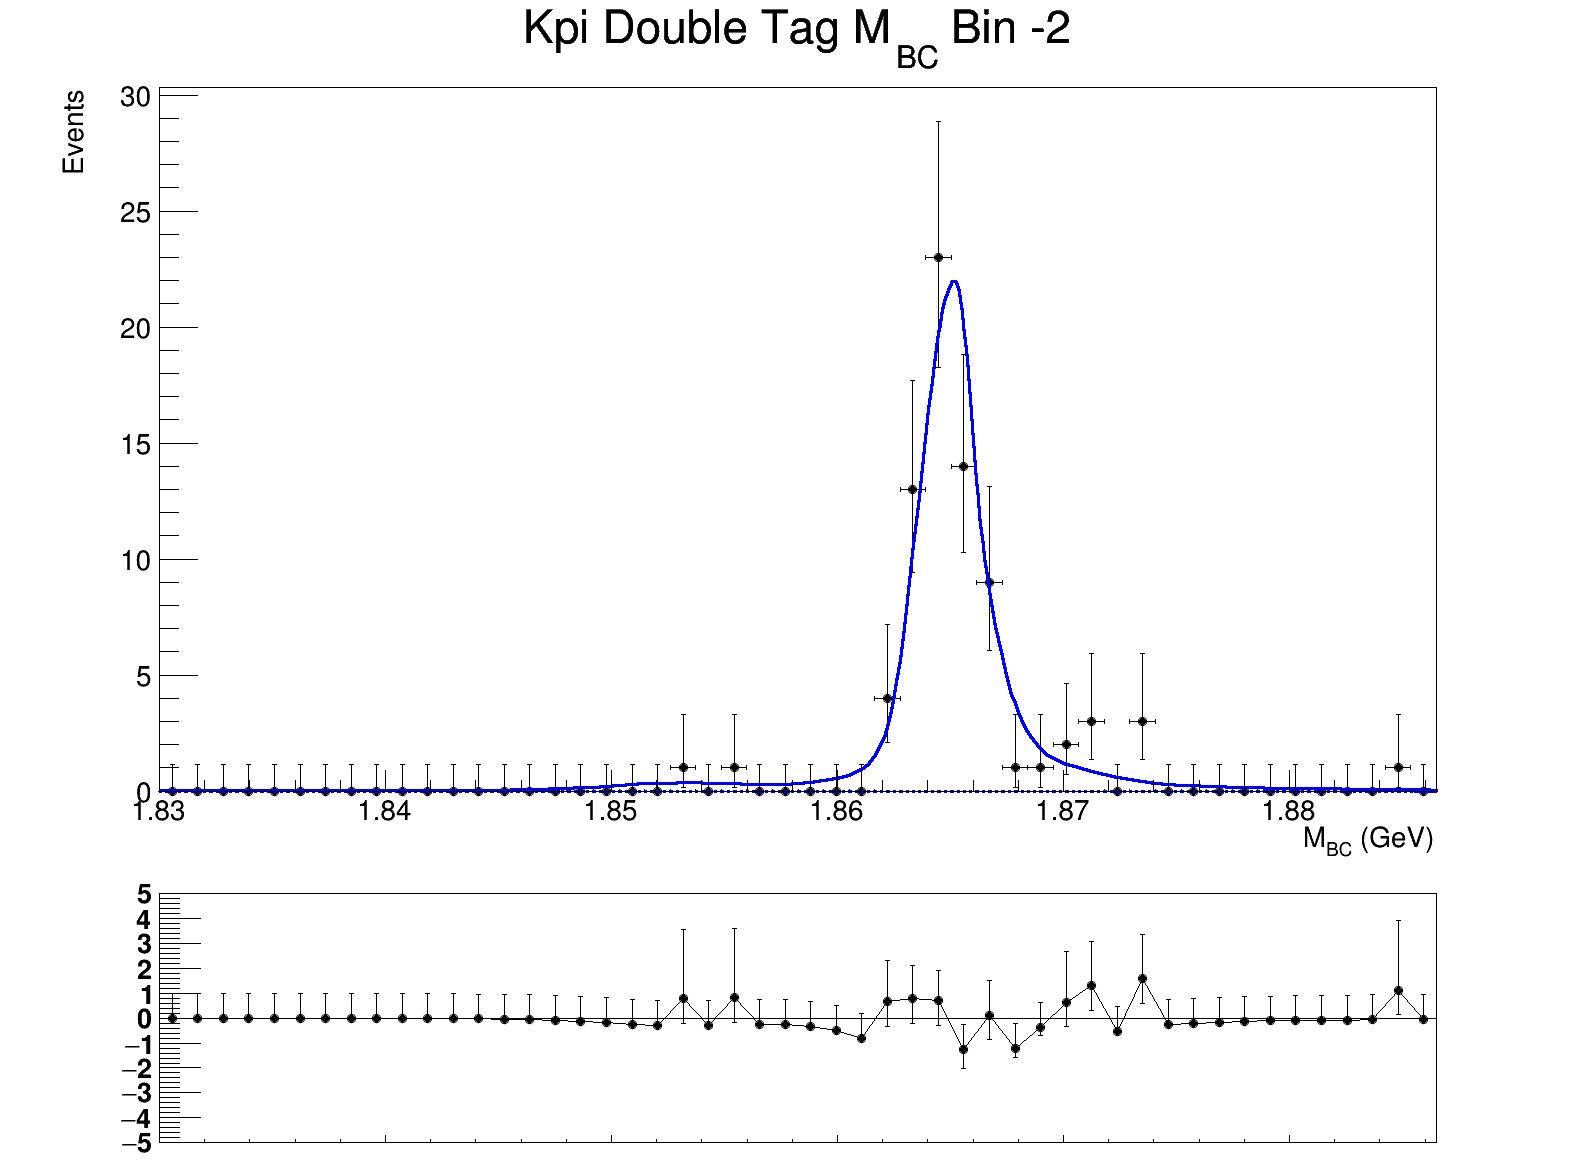
\includegraphics[width=\textwidth]{Plots/DoubleTagYield_DoubleTag_Flavour_KKpipi_vs_Kpi_SignalBinM2_TagBin0.png}
      \caption{Bin $-2$}
    \end{subfigure}%
    \begin{subfigure}{0.38\textwidth}
      \centering
      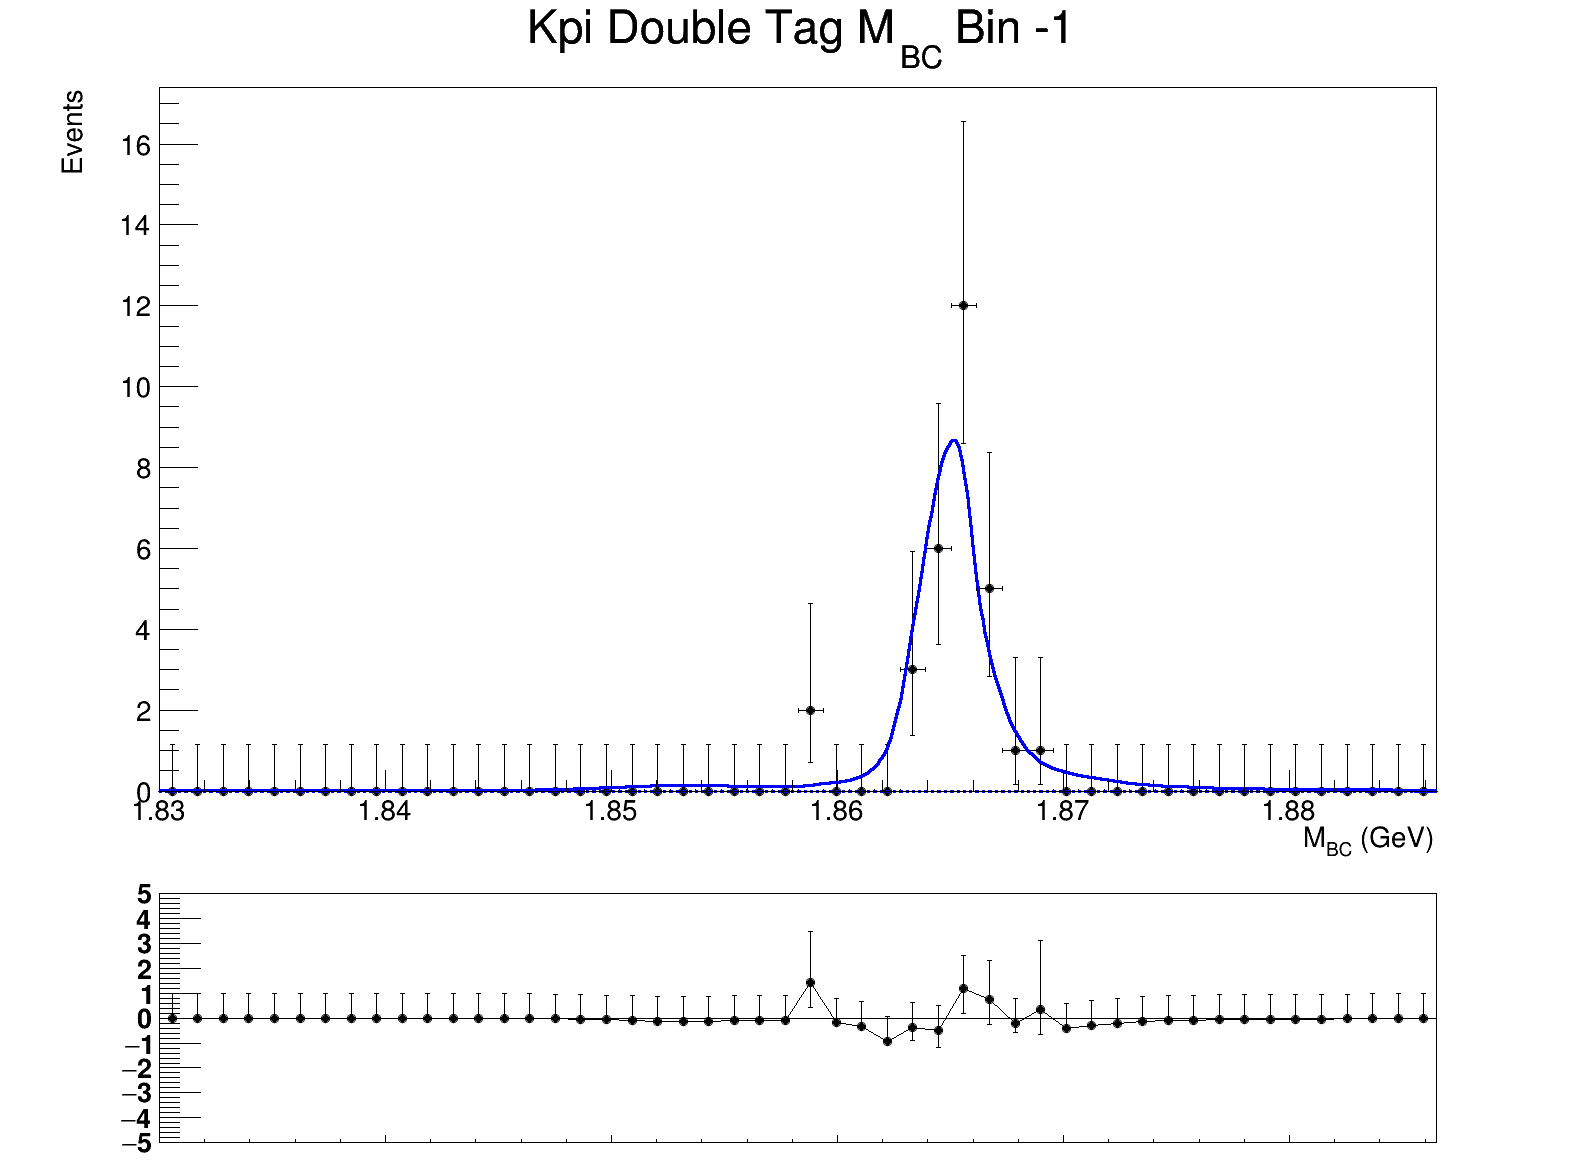
\includegraphics[width=\textwidth]{Plots/DoubleTagYield_DoubleTag_Flavour_KKpipi_vs_Kpi_SignalBinM1_TagBin0.png}
      \caption{Bin $-1$}
    \end{subfigure}
  \end{figure}
\end{frame}

\begin{frame}{Double tag yield simultaneous fit ($KK\pi\pi$ vs $K\pi$)}
  \begin{figure}
    \centering
    \begin{subfigure}{0.38\textwidth}
      \centering
      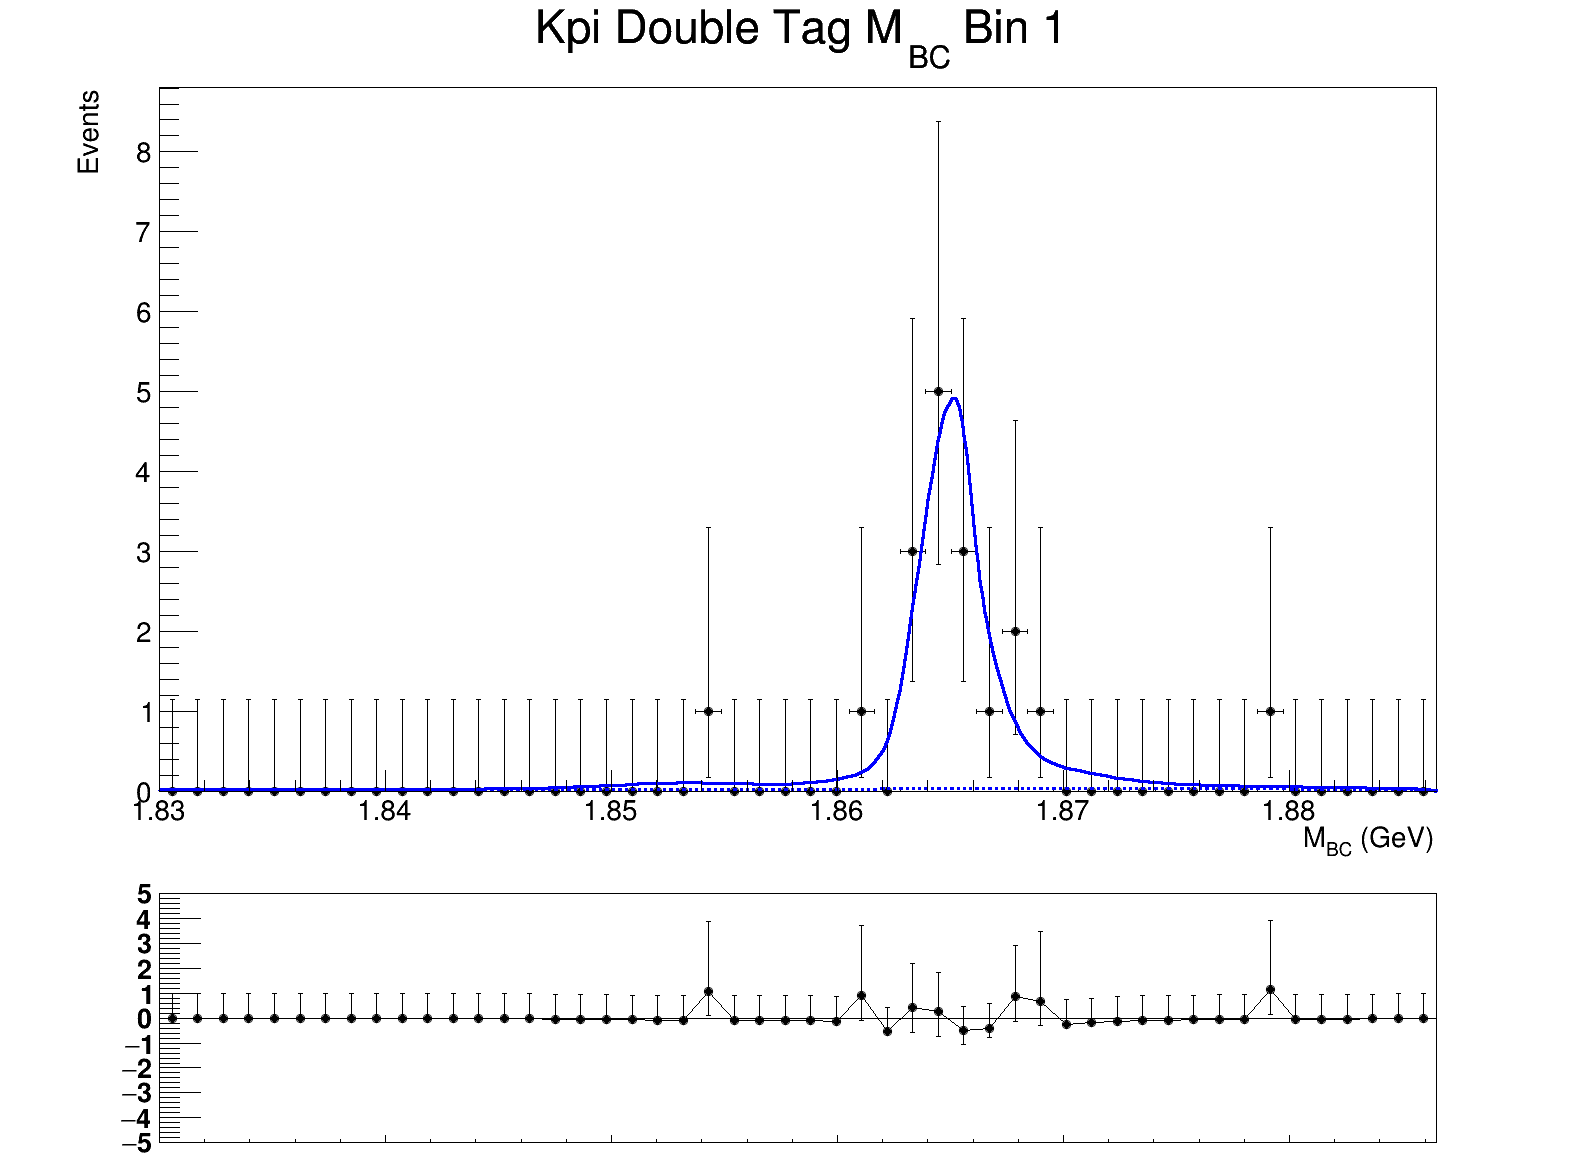
\includegraphics[width=\textwidth]{Plots/DoubleTagYield_DoubleTag_Flavour_KKpipi_vs_Kpi_SignalBinP1_TagBin0.png}
      \caption{Bin $1$}
    \end{subfigure}%
    \begin{subfigure}{0.38\textwidth}
      \centering
      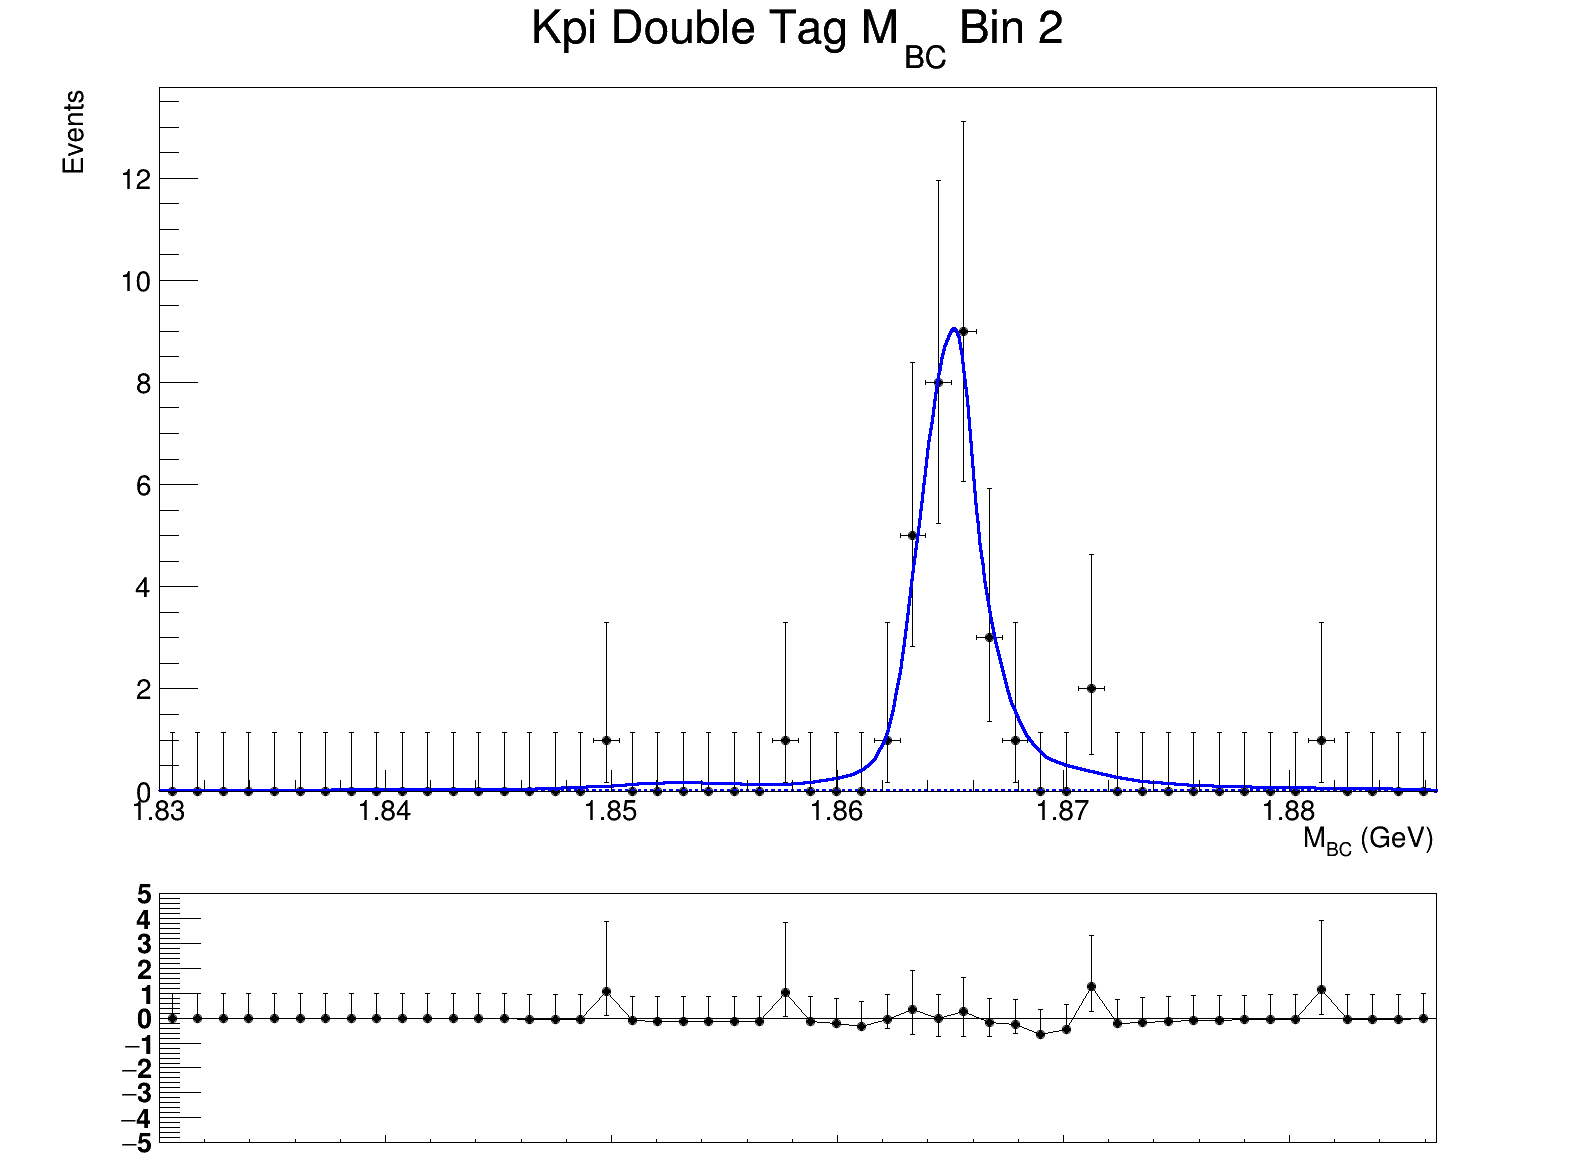
\includegraphics[width=\textwidth]{Plots/DoubleTagYield_DoubleTag_Flavour_KKpipi_vs_Kpi_SignalBinP2_TagBin0.png}
      \caption{Bin $2$}
    \end{subfigure}
    \begin{subfigure}{0.38\textwidth}
      \centering
      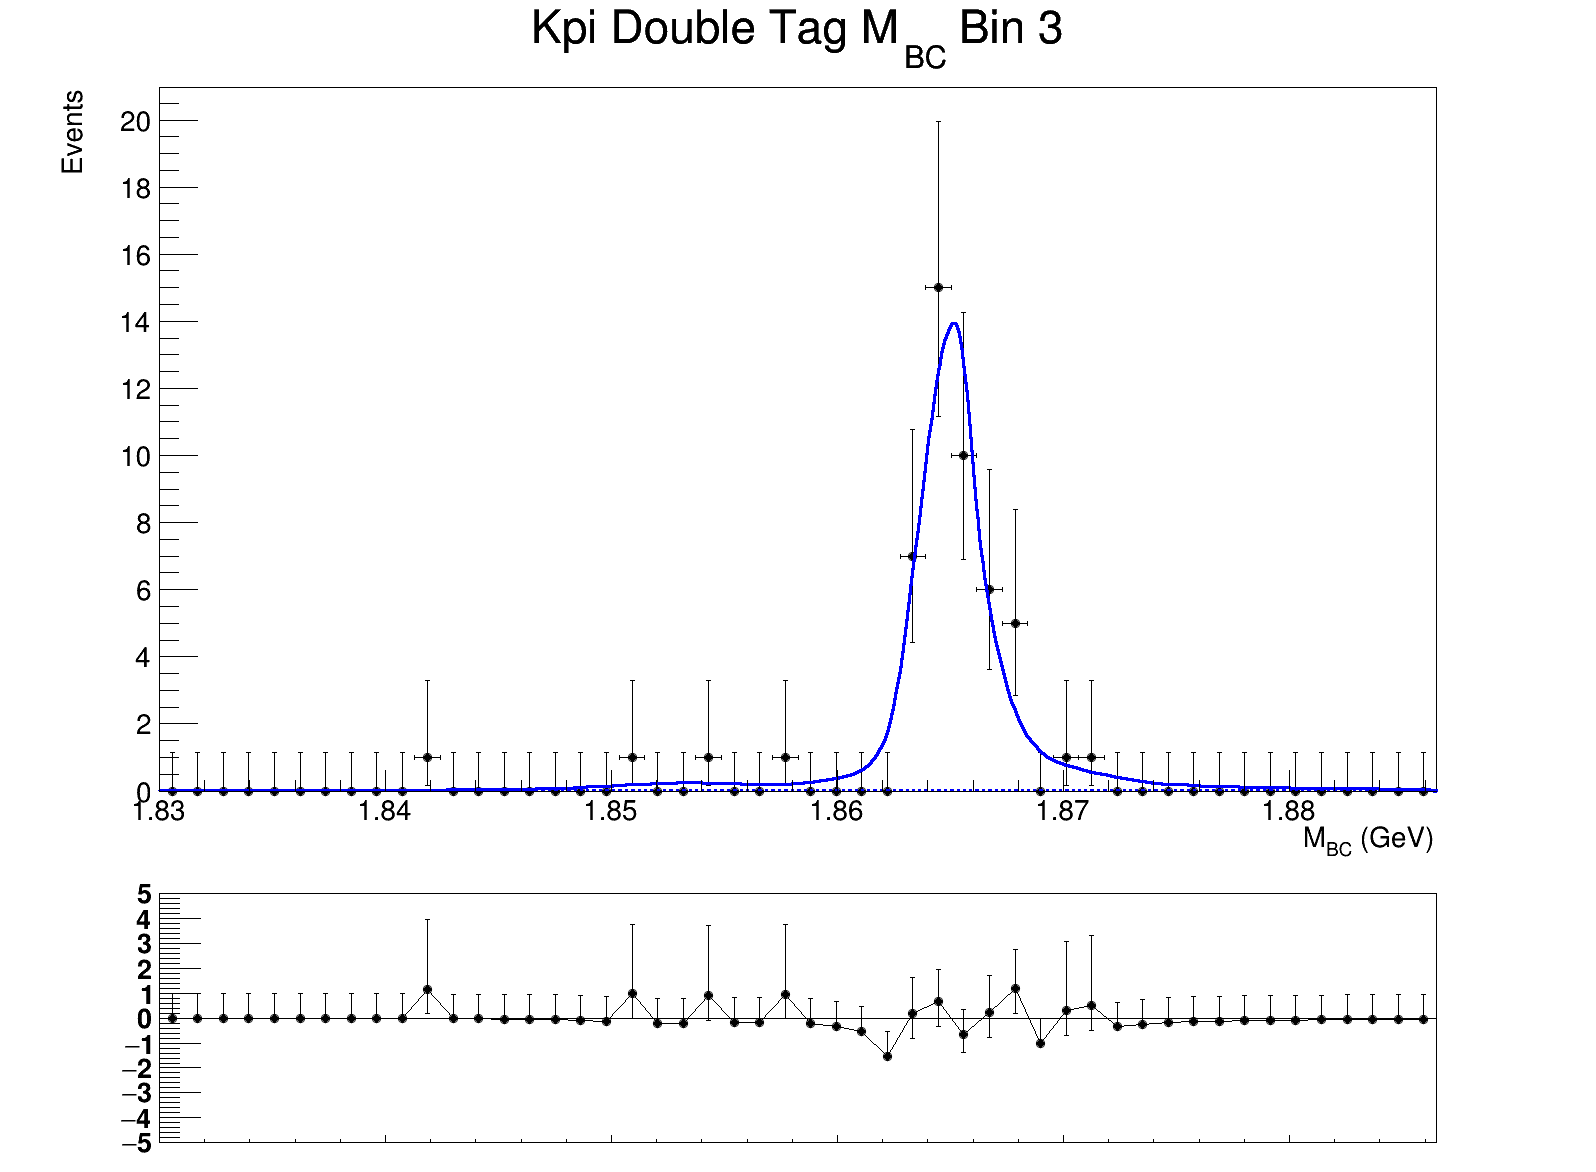
\includegraphics[width=\textwidth]{Plots/DoubleTagYield_DoubleTag_Flavour_KKpipi_vs_Kpi_SignalBinP3_TagBin0.png}
      \caption{Bin $3$}
    \end{subfigure}%
    \begin{subfigure}{0.38\textwidth}
      \centering
      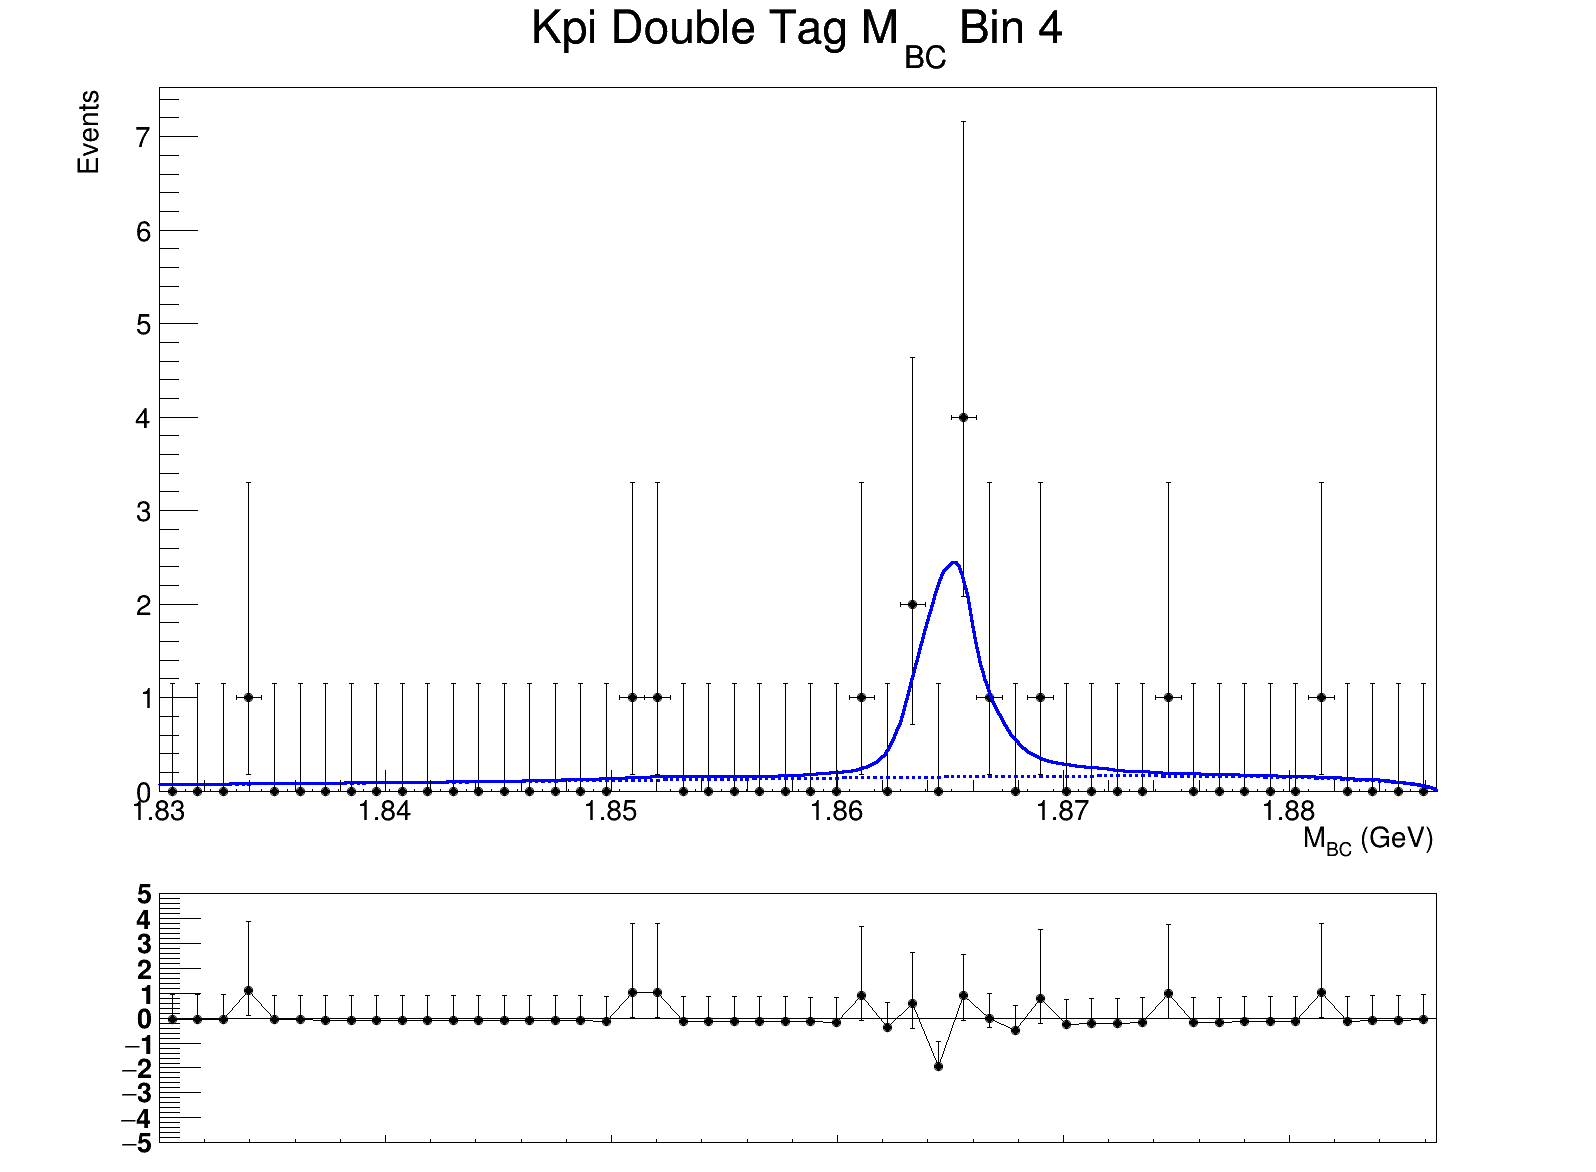
\includegraphics[width=\textwidth]{Plots/DoubleTagYield_DoubleTag_Flavour_KKpipi_vs_Kpi_SignalBinP4_TagBin0.png}
      \caption{Bin $4$}
    \end{subfigure}
  \end{figure}
\end{frame}

\section{Efficiency corrections}
\begin{frame}{Efficiency corrections}
  \begin{itemize}
    \setlength\itemsep{1.5em}
    \item{Single tag efficiencies trivially corrected by dividing the yields}
    \item{For double tags, construct an efficiency matrix to account for both efficiency and bin migration}
    \item{For events reconstructed in bin $i$ and generated in bin $j$:}
  \end{itemize}
  \begin{center}
    $\epsilon_{ij} = \frac{N^{\rm reconstructed}_{ij}}{N^{\rm generated}_j}$
  \end{center}
\end{frame}

\begin{frame}{Efficiency corrections}
  \begin{figure}
    \centering
    \begin{subfigure}{0.38\textwidth}
      \centering
      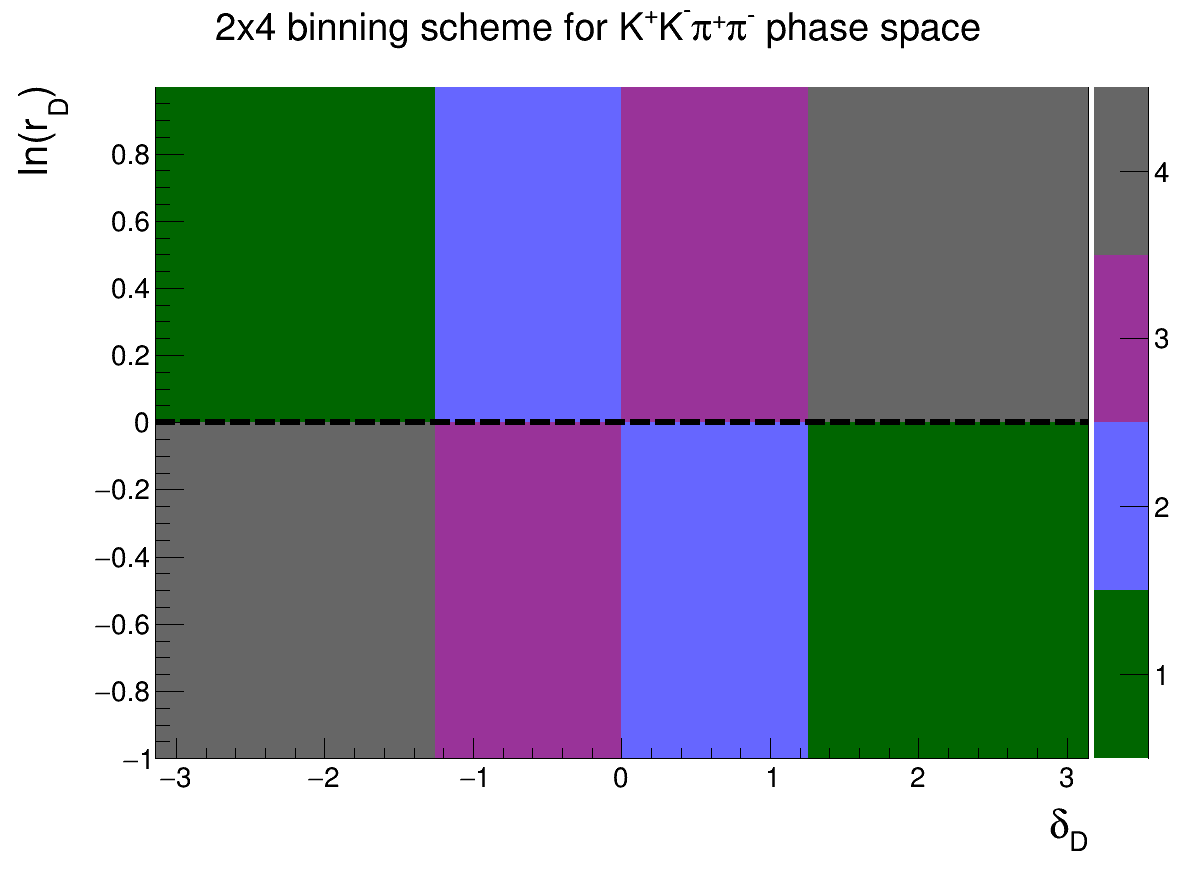
\includegraphics[width=\textwidth]{Plots/BinningSchemePlot_4Bins.png}
      \caption{Binning scheme}
    \end{subfigure}
    \begin{subfigure}{0.38\textwidth}
      \centering
      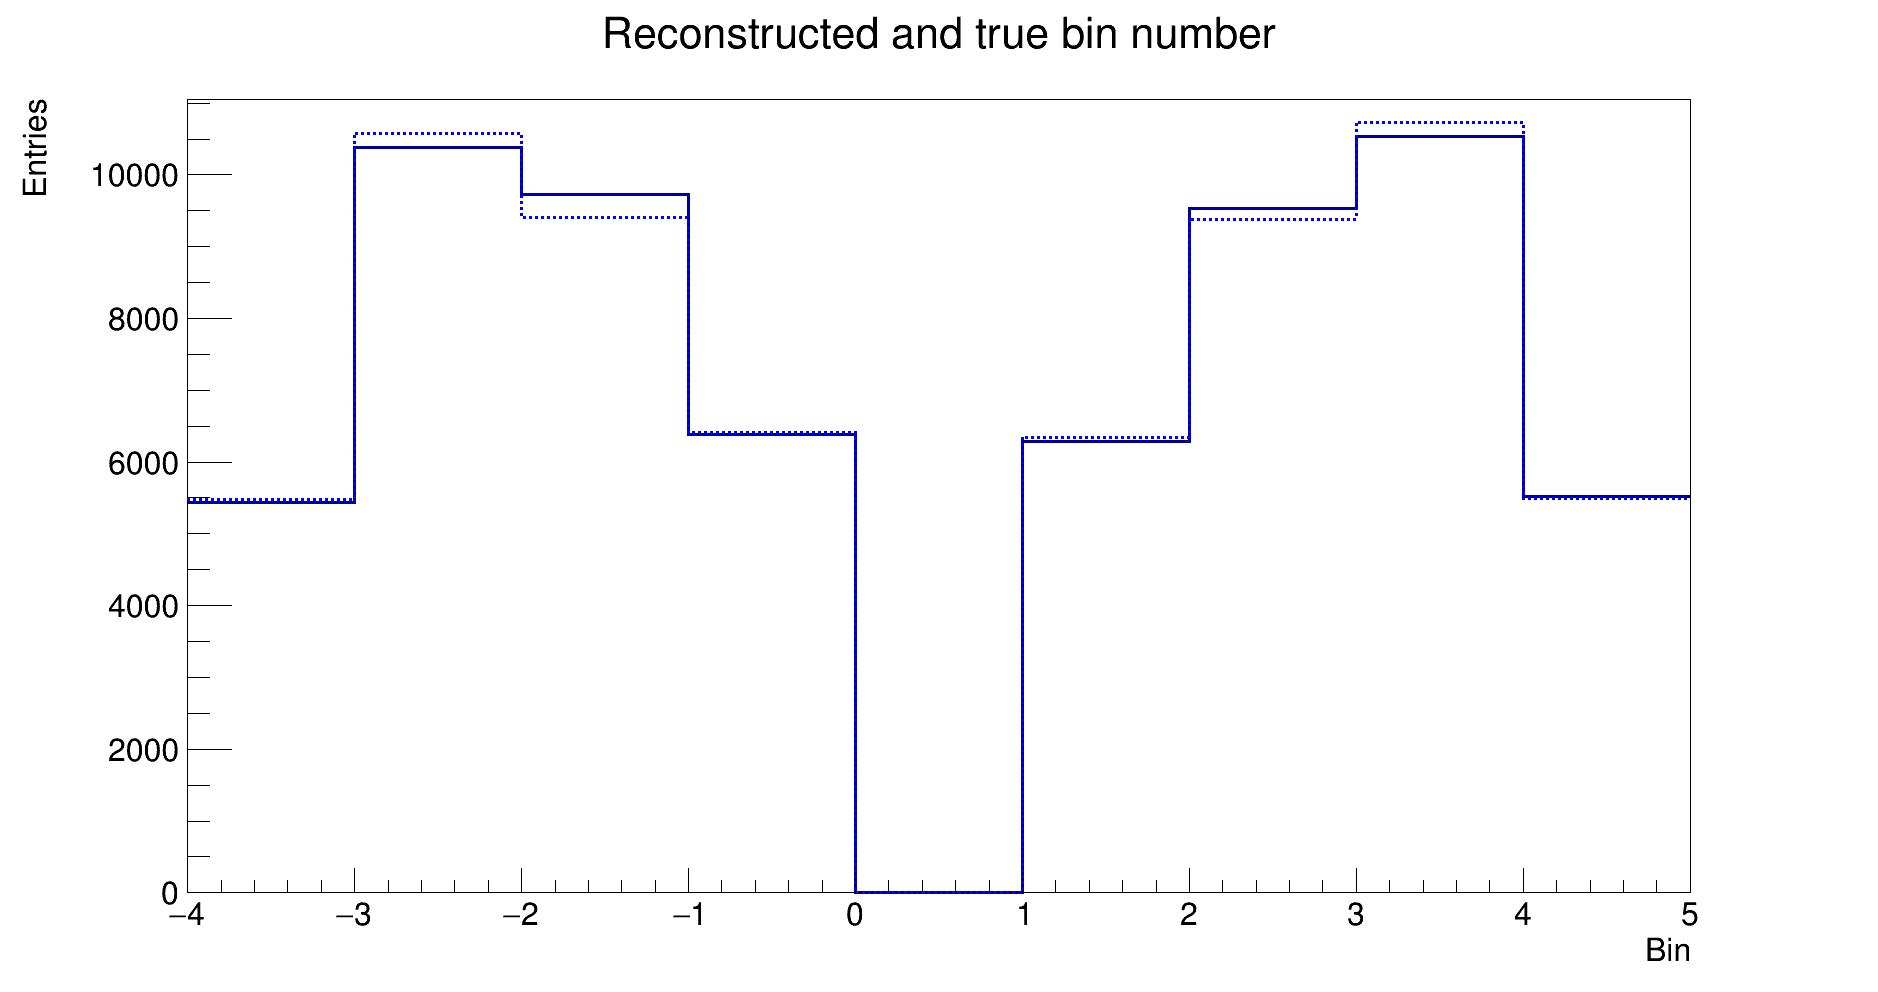
\includegraphics[width=\textwidth]{Plots/ReconstructedTrueBins.png}
      \caption{Reconstructed bin vs true bin}
    \end{subfigure}%
    \begin{subfigure}{0.38\textwidth}
      \centering
      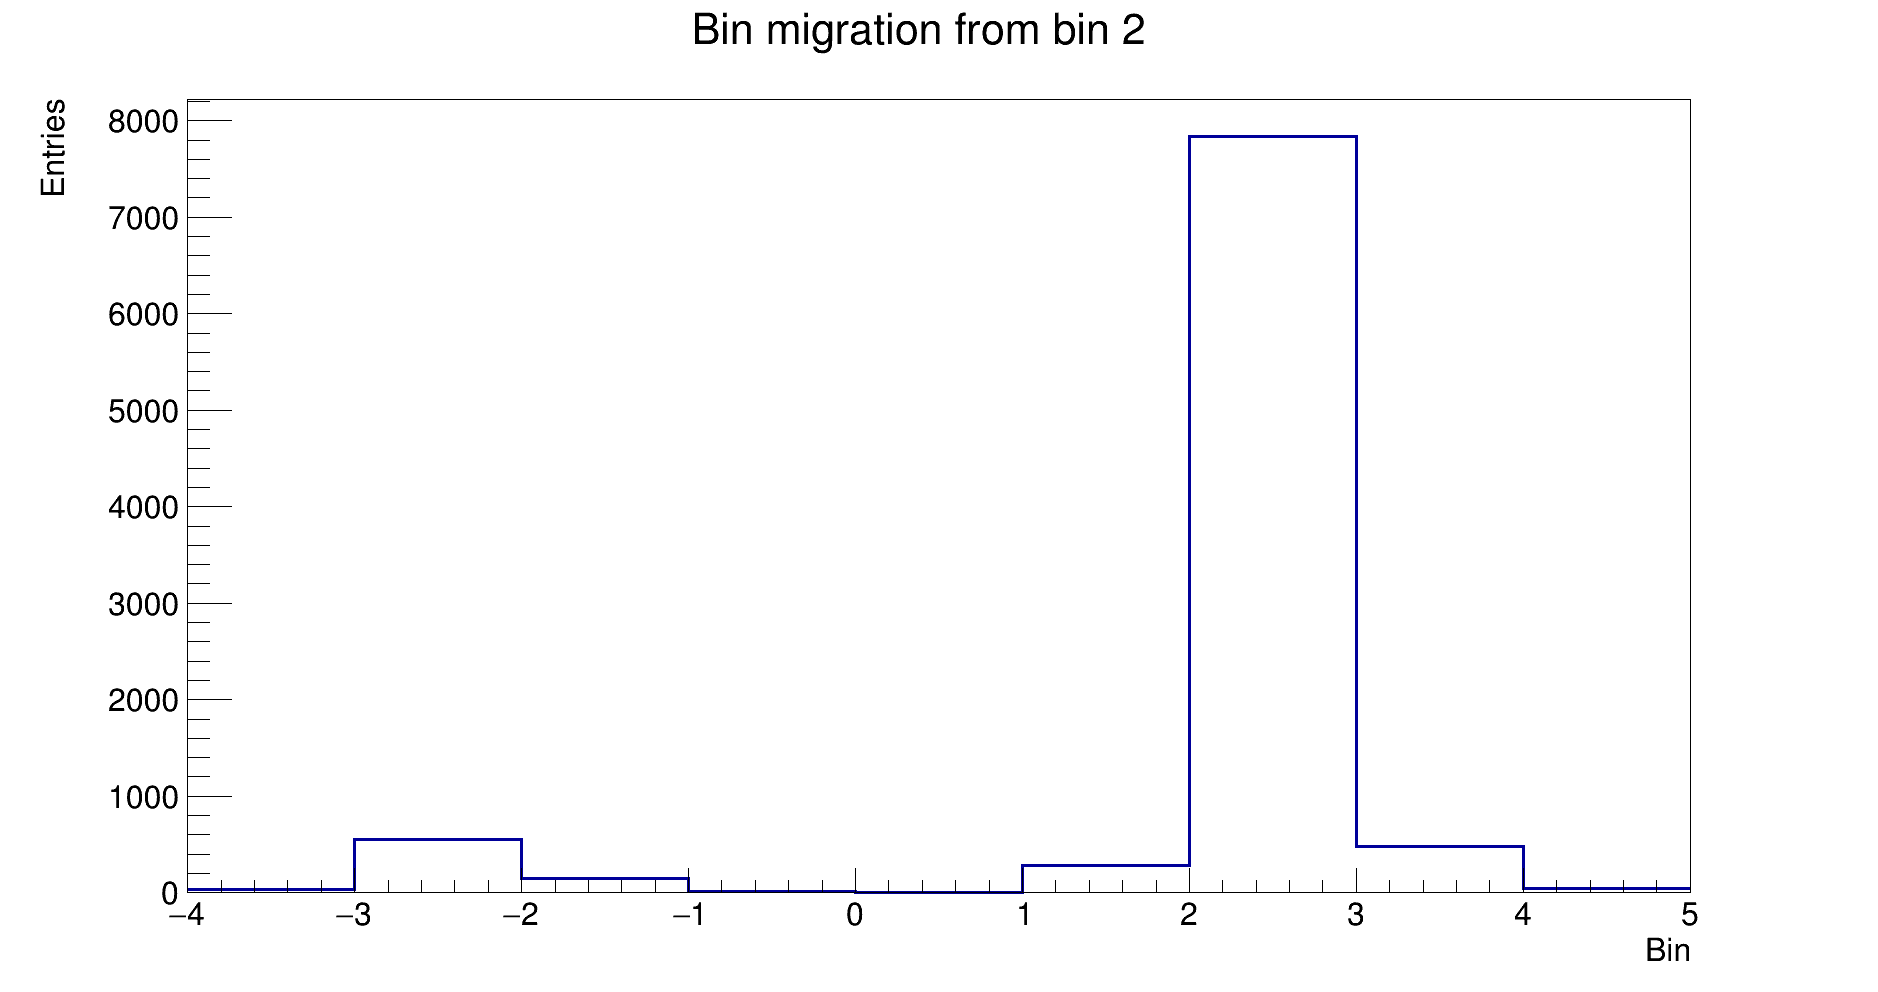
\includegraphics[width=\textwidth]{Plots/BinMigrationBin2.png}
      \caption{Bin migration from bin $2$}
    \end{subfigure}
  \end{figure}
  \begin{center}
    Bin migration much higher than expected ($10\%$-$15\%$) \\
    But net migration is relatively small
  \end{center}
\end{frame}

\section{DCS corrections}
\begin{frame}{DCS corrections}
  \begin{center}
    Calculate using $c_i$, $s_i$, $K_i$ from LHCb model
  \end{center}
  \centering
  \def\arraystretch{1.2}%
  \begin{tabular}{c|c}
    Bin           & Correction \\
    \hline
    $-4$          &$\SI{1.0091(17)}{}$ \\
    $-3$          &$\SI{0.9538(7)}{}$ \\
    $-2$          &$\SI{0.9669(14)}{}$ \\
    $-1$          &$\SI{1.0166(16)}{}$ \\
    $+1$          &$\SI{1.0599(228)}{}$ \\
    $+2$          &$\SI{0.7833(27)}{}$ \\
    $+3$          &$\SI{0.8263(60)}{}$ \\
    $+4$          &$\SI{1.1850(229)}{}$ \\
    \hline
  \end{tabular}
\end{frame}

\section{\texorpdfstring{$K_i$}{Ki} results for \texorpdfstring{$KK\pi\pi$}{KKpipi} vs \texorpdfstring{$K\pi$}{Kpi}}
\begin{frame}{$K_i$ results for $KK\pi\pi$ vs $K\pi$}
  \begin{figure}
    \centering
    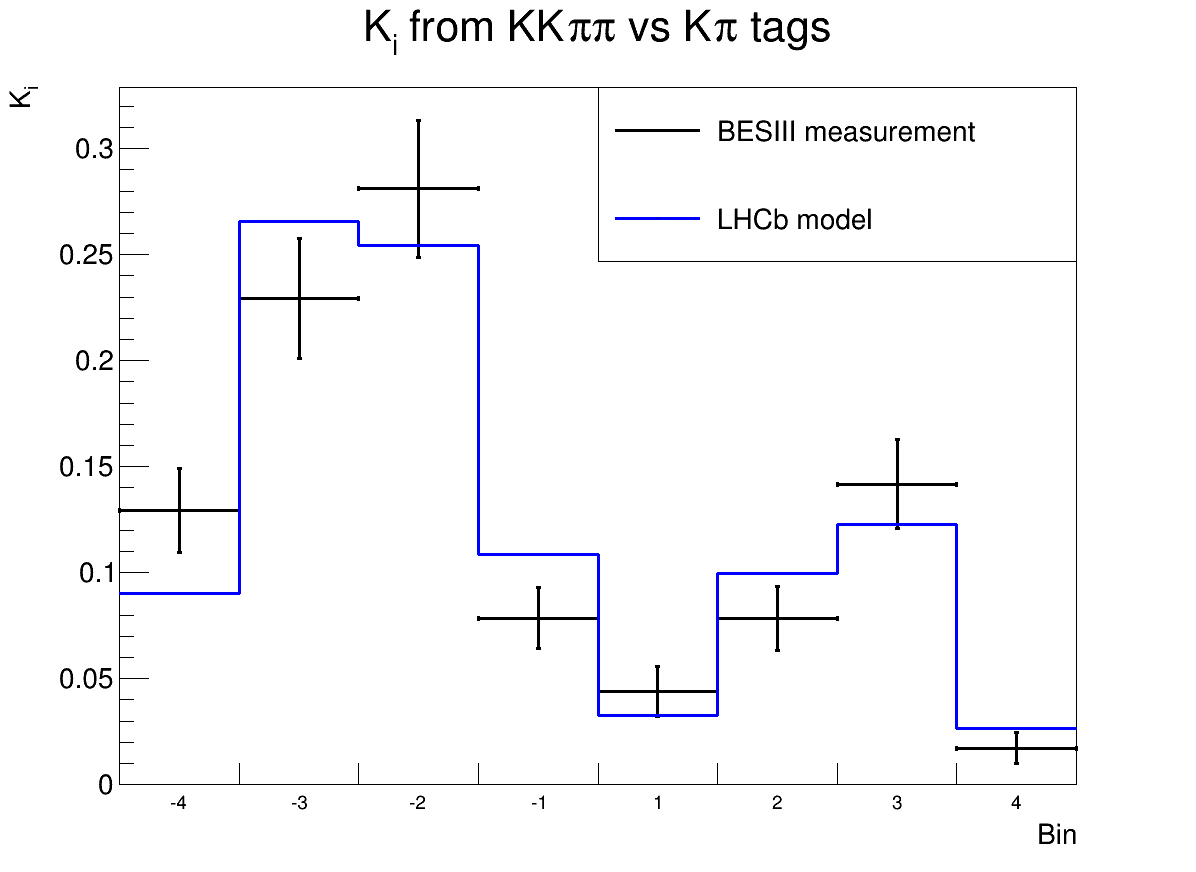
\includegraphics[width=0.9\textwidth]{Plots/Kpi_Ki.png}
  \end{figure}
\end{frame}

\section{Next steps}
\begin{frame}{Conclusion and next steps}
  \begin{itemize}
    \setlength\itemsep{1.5em}
    \item{Single tag $m_{\rm BC}$ show acceptable fit quality now}
    \item{Double tag simultaneous fit works great!}
    \item{$K_i$ from $KK\pi\pi$ vs $K\pi$ tag looks encouraging, but not perfect}
    \item{Next steps:}
    \begin{itemize}
      \item{Include $K\pi\pi^0$, $K\pi\pi\pi$ and $Ke\nu$ tags in $K_i$ determination}
      \item{Calculate peaking backgrounds in each bin with LHCb model}
      \item{Develop likelihood fitter for $c_i$/$s_i$ and run some toys}
      \item{Start looking at CP tag fits to data (but yields will be very low!)}
      \item{Remove $K_S\phi$, include $K_SKK$ and $K_LKK$ as self-conjugate tags}
    \end{itemize}
  \end{itemize}
\end{frame}

\end{document}
